% (c) 2012 -2014 Dimitrios Vrettos - d.vrettos@gmail.com
\chapter{Generalità sugli insiemi}
\section{Insiemi ed elementi}

In matematica usiamo la parola \textit{insieme} per indicare un
raggruppamento, una collezione, una raccolta di oggetti, individui,
simboli, numeri, figure che sono detti \textit{elementi}
dell'insieme e che sono ben definiti e distinti tra di
loro.

La nozione di insieme e quella di elemento di un insieme in matematica
sono considerate nozioni primitive, nozioni che si preferisce non
definire mediante altre più semplici.

\begin{exrig}
 \begin{esempio}
 Sono insiemi:
 \begin{enumeratea}
  \item l'insieme delle lettere della parola RUOTA;
  \item l'insieme delle canzoni che ho ascoltato la settimana scorsa;
  \item l'insieme delle città della Puglia con più di~$\np{15000}$ abitanti;
  \item l'insieme delle lettere dell'alfabeto italiano;
  \item l'insieme dei numeri~1, 2, 3, 4, 5;
  \item l'insieme delle montagne d'Italia più alte di~$\np{1000}$ metri.
 \end{enumeratea}
 \end{esempio}
\end{exrig}

Per poter assegnare un insieme occorre soddisfare le seguenti condizioni:

\begin{itemize*}
\item bisogna poter stabilire con certezza e oggettività se un oggetto
è o non è un elemento dell'insieme;
\item gli elementi di uno stesso insieme devono essere differenti tra
loro, cioè un elemento non può essere ripetuto più volte nello stesso insieme.
\end{itemize*}

Non possono essere considerati insiemi:
\begin{itemize*}
 \item i film interessanti (non c'è un criterio oggettivo per stabilire se un film è interessante oppure no, uno stesso film
può risultare interessante per alcune persone e non interessante per altre);
 \item le ragazze simpatiche di una classe (non possiamo stabilire in maniera oggettiva se una ragazza è simpatica);
 \item le montagne più alte d'Italia (non possiamo dire se una montagna è tra le più alte poiché non è fissata
un'altezza limite);
 \item l'insieme delle grandi città d'Europa (non c'è un criterio per
stabilire se una città è grande);
\end{itemize*}

\ovalbox{\risolvi \ref{ese:5.1}}\vspazio


In generale, gli insiemi si indicano con lettere maiuscole~$A$, $B$, $C$, \ldots e
gli elementi con lettere minuscole~$a$, $b$, $c$, \ldots

Se un elemento~$a$ sta nell'insieme~$A$ si scrive~$a\in A$ e si legge ``$a$ appartiene ad~$A$''.
Il simbolo ``$\in$'' si chiama simbolo di \textit{appartenenza}.

Se un elemento~$b$ non sta nell'insieme~$A$ si scrive~$b\notin A$ e
si legge ``$b$ non appartiene ad~$A$''. Il simbolo ``$\notin$''
si chiama simbolo di \textit{non appartenenza}.

Il criterio che stabilisce se un elemento appartiene a un insieme si chiama \textit{proprietà caratteristica} dell'insieme.

Un altro modo per definire un insieme, oltre a quello di indicare la sua proprietà caratteristica, è quello di elencare i suoi elementi separati da virgole e racchiusi tra parentesi graffe. Ad esempio: $A=\{a\text{, }b\text{, }c\text{, }d\}$.

Per indicare alcuni insiemi specifici vengono utilizzati simboli particolari:
\begin{itemize*}
 \item $\insN$ si utilizza per indicare l'insieme dei numeri naturali:~$\insN=\{0\text{, }1\text{, }2\text{, }3\text{, }\ldots\}$;
 \item $\insZ$ si utilizza per indicare i numeri interi relativi:~$\insZ=\{\ldots\text{, }-2\text{, }-1\text{, }0\text{, }+1\text{, }+2\text{, }\ldots\}$;
 \item $\insQ$ si utilizza per indicare i numeri razionali:~$\insQ=\{\dfrac{1}{2}\text{, }-\dfrac{3}{5}\text{, }\dfrac{5}{1}\text{, }-\dfrac{4}{17}\text{, }\np{12,34}\text{, }8\text{, }\np{0,}\overline{25}\text{, }\ldots\}$.
 \end{itemize*}


 \begin{exrig}
 \begin{esempio}
Indica con il simbolo opportuno quali dei seguenti elementi appartengono
o non appartengono all'insieme $A$ dei giorni della
settimana: lunedì, martedì, gennaio, giovedì, dicembre, estate.

Gennaio e dicembre sono mesi dell'anno, perciò scriviamo:
\[\text{lunedì}\in A\text{,\:}\text{martedì}\in A\text{,\:}\text{gennaio}\notin A\text{,\:}\text{giovedì}\in A\text{,\:}\text{dicembre}\notin A\text{,\:}\text{estate}\notin A.\]
 \end{esempio}
\end{exrig}

Consideriamo l'insieme~$A=\{\text{r, s, t}\}$ e l'insieme~$B$ delle consonanti della parola
``risate''. Possiamo osservare che~$A$ e~$B$ sono due insiemi costituiti dagli stessi
elementi; diremo che sono \textit{insiemi uguali}.

\begin{definizione}
 Due insiemi~$A$ e~$B$ si dicono \emph{uguali} se sono formati dagli stessi elementi, anche se
disposti in ordine diverso. In simboli si scrive~$A=B$. Altrimenti i due insiemi si dicono \emph{diversi}, in simboli~$A\neq B$.
\end{definizione}

\ovalbox{\risolvii \ref{ese:5.2}, \ref{ese:5.3}, \ref{ese:5.4}, \ref{ese:5.5}, \ref{ese:5.6}, \ref{ese:5.7}, \ref{ese:5.8}, \ref{ese:5.9}}

\section{Insieme vuoto, insieme universo, cardinalità}\label{sect:universo}

Consideriamo l'insieme~$A=\{\text{consonanti della parola ``AIA''}\}$. Poiché la parola ``AIA'' non
contiene consonanti, l'insieme~$A$ è privo di elementi.

\begin{definizione}
 Un insieme privo di elementi si chiama \emph{insieme vuoto} e lo si indica con il simbolo~$\emptyset$ o $\{ \}$.
\end{definizione}

\osservazione $\{ \}=\emptyset$ ma~$\{\emptyset \}\neq\emptyset$ dato che la scrittura~$\{\emptyset \}$ rappresenta un insieme che ha
come unico elemento l'insieme vuoto.

\begin{exrig}
 \begin{esempio}
 Alcuni insiemi vuoti.
 \begin{enumeratea}
  \spazielenx
\item L'insieme dei numeri negativi maggiori di~5 è vuoto;
\item l'insieme delle capitali europee con meno di~50 abitanti è vuoto;
\item l'insieme dei numeri naturali minori di~0 è vuoto.
 \end{enumeratea}
 \end{esempio}
\end{exrig}

La frase <<l'insieme degli studenti che vengono a scuola con il motorino>> non definisce un
insieme particolare. Occorre definire il contesto, l'ambiente che fa individuare gli elementi
dell'insieme. Se l'ambiente è la classe~1\textsuperscript{a}C gli elementi considerati saranno certamente diversi, e probabilmente meno numerosi, di quelli che compongono l'ambiente di un'intera scuola o di un'intera
città. Quando si identifica un insieme, occorre indicare anche l'ambiente di riferimento da cui trarre gli elementi che appartengono al nostro insieme. Questo insieme si chiama \emph{insieme universo} e rappresenta il contesto, l'ambiente su cui faremo le nostre osservazioni. In generale l'insieme universo per un insieme~$A$ è semplicemente un insieme che contiene~$A$. Solitamente l'insieme universo viene indicato con~$U$.

\subsection{Cardinalità}

\begin{definizione}
 Si definisce \emph{cardinalità} (o \emph{potenza}) di un insieme finito il numero
degli elementi dell'insieme. Essa viene indicata con uno dei seguenti simboli~$\valass{A}$, \#($A$) o~$\card(A)$.
\end{definizione}

Per poter parlare di cardinalità di un insieme qualsiasi, che
comprenda anche insiemi infiniti come gli insiemi numerici, occorre una
definizione più complessa che qui non daremo.

\begin{exrig}
 \begin{esempio}
 Esempi di cardinalità.
 \begin{enumeratea}
  \item L'insieme~$A$ delle vocali dell'alfabeto italiano ha~5 elementi, quindi~$\card(A)=5$;
  \item l'insieme~$B$ dei multipli di~3 minori di~10 ha~3 elementi, quindi~$\card(B)=3$.
 \end{enumeratea}
 \end{esempio}
\end{exrig}

\ovalbox{\risolvii \ref{ese:5.10}, \ref{ese:5.11}, \ref{ese:5.12}, \ref{ese:5.13}, \ref{ese:5.14}, \ref{ese:5.15}}

\newpage
% (c) 2012 Dimitrios Vrettos - d.vrettos@gmail.com
% (c) 2012 Claudio Carboncini - claudio.carboncini@gmail.com
\section{Esercizi}
\subsection{Esercizi dei singoli paragrafi}
\subsubsection*{\thechapter.1 - Insiemi ed elementi}

\begin{esercizio}
 \label{ese:\thechapter.1}
 Barra con una crocetta i raggruppamenti che ritieni siano degli insiemi.
 \begin{multicols}{2}
 \begin{enumeratea}
\item I fiumi più lunghi d'Italia;
\item le persone con più di~30 anni;
\item i numeri~1, 20, 39, 43, 52;
\item i libri più pesanti nella tua cartella;
\item i punti di una retta;
\item gli animali con~2 zampe;
\item le vocali dell'alfabeto italiano;
\item i professori bravi;
\item i gatti con due code;
\item i calciatori che hanno fatto pochi gol.
\end{enumeratea}
\end{multicols}
\end{esercizio}

%%%%%%%%%%%%%%%%%%%%%%%%%%%%%%%%%%%%%%%%%%%%%%%%%%%%%%%%%%%%%%%%%%%%%
\begin{esercizio}
 \label{ese:\thechapter.2}
Considerando l'insieme $A$ delle lettere dell'alfabeto italiano, per ciascuno dei seguenti casi inserisci il simbolo adatto fra ``$\in$'' e ``$\notin$''.

b \ldots $A$, i \ldots $A$, j \ldots $A$, e \ldots $A$, w \ldots $A$, z \ldots $A$.
\end{esercizio}

\begin{esercizio}
\label{ese:\thechapter.3}
Le vocali delle parole che seguono formano insiemi uguali, tranne in un caso. Quale?
\begin{center}
 \boxA\quad sito\quad\boxB\quad micio\quad\boxC\quad zitto\quad\boxD\quad fiocco\quad\boxE\quad lecito\quad\boxF\quad dito.
\end{center}
\end{esercizio}

\begin{esercizio}
\label{ese:\thechapter.4}
Individua tra i seguenti insiemi quelli che sono uguali:
\begin{multicols}{2}
\begin{enumeratea}
 \item vocali della parola ``SASSO'';
 \item consonanti della parola ``SASSO'';
 \item vocali della parola ``PIETRA'';
 \item vocali della parola ``PASSO''.
\end{enumeratea}
\end{multicols}
\end{esercizio}

\begin{esercizio}
\label{ese:\thechapter.5}
Quali delle seguenti frasi rappresentano criteri oggettivi per individuare un insieme? Spiega perché.
\TabPositions{8.5cm}
\begin{enumeratea}
\item Le città che distano meno di~100 km da Lecce; \tab\boxV\quad\boxF
\item i laghi d'Italia;  \tab\boxV\quad\boxF
\item le città vicine a Roma; \tab\boxV\quad\boxF
\item i calciatori della Juventus;  \tab\boxV\quad\boxF
\item i libri di Mauro;  \tab\boxV\quad\boxF
\item i professori bassi della tua scuola;  \tab\boxV\quad\boxF
\item i tuoi compagni di scuola il cui nome inizia per M; \tab\boxV\quad\boxF
\item i tuoi compagni di classe che sono gentili; \tab\boxV\quad\boxF
\item gli zaini neri della tua classe.  \tab\boxV\quad\boxF
\end{enumeratea}
\end{esercizio}

\begin{esercizio}
\label{ese:\thechapter.6}
Scrivi al posto dei puntini il simbolo mancante tra ``$\in$'' e ``$\notin$''.

\begin{enumeratea}
\item La Polo \ldots\ldots all'insieme delle automobili Fiat;
\item il cane \ldots\ldots all'insieme degli animali domestici;
\item la Puglia \ldots\ldots all'insieme delle regioni italiane;
\item Firenze \ldots\ldots all'insieme delle città francesi;
\item il numero~10 \ldots\ldots all'insieme dei numeri naturali;
\item il numero~3 \ldots\ldots all'insieme dei numeri pari.
\end{enumeratea}
\end{esercizio}
\pagebreak
\begin{esercizio}
\label{ese:\thechapter.7}
Quali delle seguenti proprietà sono caratteristiche per un insieme?
\TabPositions{8.5cm}
\begin{enumeratea}
\item Essere una città italiana il cui nome inizia per W; \tab\boxV\quad\boxF
\item essere un bravo cantante; \tab\boxV\quad\boxF
\item essere un monte delle Alpi;  \tab\boxV\quad\boxF
\item essere un ragazzo felice; \tab\boxV\quad\boxF
\item essere un numero naturale grande;\tab\boxV\quad\boxF
\item essere un ragazzo nato nel~1985; \tab\boxV\quad\boxF
\item essere un alunno della classe~1\textsuperscript{a}C; \tab\boxV\quad\boxF
\item essere una lettera dell'alfabeto inglese; \tab\boxV\quad\boxF
\item essere una retta del piano; \tab\boxV\quad\boxF
\item essere un libro interessante della biblioteca; \tab\boxV\quad\boxF
\item essere un italiano vivente nato nel~1850; \tab\boxV\quad\boxF
\item essere un italiano colto. \tab\boxV\quad\boxF
\end{enumeratea}
\end{esercizio}

\begin{esercizio}
\label{ese:\thechapter.8}
Le stelle dell'universo formano un insieme. Le stelle visibili a occhio nudo formano un insieme? Spiega il tuo punto di vista.
\end{esercizio}

\subsubsection*{\thechapter.2 - Insieme vuoto, insieme universo, cardinalità}
\begin{esercizio}
\label{ese:\thechapter.9}
Indica se gli insiemi~$G =\{\text{gatti con~6 zampe}\}$ e~$P = \{\text{polli con~2 zampe}\}$ sono o non sono vuoti.
\end{esercizio}

\begin{esercizio}
\label{ese:\thechapter.10}
Barra con una croce gli insiemi vuoti.
\begin{enumeratea}
 \item L'insieme dei numeri positivi minori di~0;
 \item l'insieme dei numeri negativi minori di~100;
 \item l'insieme dei numeri pari minori di~100;
 \item l'insieme delle capitali europee della regione Lombardia;
 \item l'insieme dei triangoli con quattro angoli;
 \item l'insieme delle capitali italiane del Lazio;
 \item l'insieme dei punti di intersezione di due rette parallele.
 \end{enumeratea}
\end{esercizio}

\begin{esercizio}
\label{ese:\thechapter.11}
Quali delle seguenti scritture sono corrette per indicare
l'insieme vuoto?
\begin{center}
 \boxA\quad~$\emptyset $ \quad\boxB\quad~0 \quad\boxC\quad~$\{\emptyset \}$ \quad\boxD\quad~$\{0\}$ \quad\boxE\quad \{ \}.
\end{center}
\end{esercizio}
\pagebreak
\begin{esercizio}
\label{ese:\thechapter.12}
Quali dei seguenti insiemi sono vuoti? Per gli insiemi non vuoti indica la cardinalità, ossia il numero di elementi che contiene.
\begin{enumeratea}
\item L'insieme degli uccelli con~6 ali;
\item l'insieme delle lettere della parola ``VOLPE'';
\item l'insieme dei cani con~5 zampe;
\item l'insieme delle vocali della parola ``COCCODRILLO'';
\item l'insieme delle vocali dell'alfabeto italiano;
\item l'insieme degli abitanti della luna;
\item l'insieme dei numeri sulla tastiera del telefonino.
\end{enumeratea}
\end{esercizio}

\begin{esercizio}
\label{ese:\thechapter.13}
Scrivi per ciascun insieme un possibile insieme universo.
\begin{enumeratea}
\item l'insieme dei rettangoli;
\item l'insieme dei multipli di~3;
\item l'insieme delle lettere della parola ``MATEMATICA'';
\item l'insieme dei libri di matematica;
\item l'insieme dei ragazzi che hanno avuto un'insufficienza in matematica.
\end{enumeratea}
\end{esercizio}

\begin{esercizio}
\label{ese:\thechapter.14}
Dato l'insieme~$A = \{\text{0, 2, 5}\}$ determina se le seguenti affermazioni sono vere o false.
\TabPositions{2.5cm}
\begin{enumeratea}
\item $0\in A$. \tab\boxV\quad\boxF
\item $5\in A$. \tab\boxV\quad\boxF
\item $\emptyset \in A$. \tab\boxV\quad\boxF
\item $A\in A$. \tab\boxV\quad\boxF
\item $\np{3,5}\in A$. \tab\boxV\quad\boxF
\end{enumeratea}
\end{esercizio}

\subsubsection*{\thechapter.3 - Rappresentazione tabulare}

\begin{esercizio}
\label{ese:\thechapter.15}
Dai una rappresentazione tabulare dei seguenti insiemi
\begin{enumeratea}
 \item delle vocali della parola ``ESERCIZI'';
 \item delle lettere della parola ``RIFLETTERE'';
 \item dei numeri naturali compresi tra~6 e~12, estremi esclusi;
 \item dei numeri dispari compresi tra~10 e~20;
 \item delle lettere dell'alfabeto italiano;
 \item dei numeri naturali minori di~10;
 \item dei multipli di~7;
 \item delle preposizioni con più di due lettere;
 \item dei numeri naturali minori di~6.
\end{enumeratea}
\end{esercizio}

\begin{esercizio}
 \label{ese:\thechapter.16}
Indica in rappresentazione tabulare i seguenti insiemi.
\TabPositions{7.5cm}
\begin{enumeratea}
 \item $A=\{x\in\insN\mid x<10\}$; %\tab\dotfill
 \item $B=\{x\in\insN\mid 2\le x<5\}$; %\tab\dotfill
 \item $C=\{x\in\insN\mid 5\le x\le~10\}$; %\tab\dotfill
 \item $D=\{x\in\insN\mid 2x\le~10\}$; % \tab\dotfill
 \item $E=\{e\in\insN\mid 5\le e<10\}$; %\tab\dotfill
 \item $F=\{f\in\insN\mid f\text{ è multiplo di~3 e } f<15\}$; %\tab\dotfill
 \item $G=\{g\in\insN\mid g\text{ è una cifra del numero }121231\}$; %\tab\dotfill
 \item $H=\{h\in\insN\mid h=3n+1\text{, con }n\in\insN\}$. %\tab\dotfill
\end{enumeratea}
\end{esercizio}

\begin{esercizio}
\label{ese:\thechapter.17}
Elenca per tabulazione gli elementi di~$A=\{x\mid x\in\insN\text{, }x\text{ è pari, }x\leq10\text{, }x\neq0\}.$
\end{esercizio}

\begin{esercizio}
\label{ese:\thechapter.18}
Elenca per tabulazione gli elementi di~$L=\{l\text{ è una lettera della parola MATEMATICA}\}$.
\end{esercizio}

\subsubsection*{\thechapter.4 - Rappresentazione caratteristica}

\begin{esercizio}
\label{ese:\thechapter.19}
Descrivi mediante la proprietà caratteristica
l'insieme~$D= \{\text{S, T, U, D, I, A, R, E}\}$.
\[D=\{x\mid x\text{ è }\ldots\ldots\ldots\ldots\}\]
\end{esercizio}


\begin{esercizio}
\label{ese:\thechapter.20}
Descrivi mediante la proprietà caratteristica l'insieme
\[X=\{\text{1, 2, 3, 4, 5, 6, 7, 8, 9, 10, 11, 12, 13, 14, 15}\}.\]
\[X=\{x\in\insN\mid x\ldots\ldots\ldots\}\]
\end{esercizio}

\begin{esercizio}
\label{ese:\thechapter.21}
Descrivi mediante la proprietà caratteristica l'insieme dei numeri primi minori di~$\np{1000}$.
\end{esercizio}

\begin{esercizio}
\label{ese:\thechapter.22}
Elenca gli elementi dell'insieme~$I=\{n\in\insN\mid n\text{ è divisore di }12\}$.
\end{esercizio}

\begin{esercizio}
\label{ese:\thechapter.23}
Elenca gli elementi dell'insieme~$I=\{n\in\insN\mid n\text{ è multiplo di~3 minore di }20\}$.
\end{esercizio}

\begin{esercizio}
\label{ese:\thechapter.24}
Dato l'insieme~$A=\{\text{2, 4, 8, 16, 32, 64}\}$ quale delle seguenti proprietà caratterizzano i suoi elementi?
\begin{enumeratea}
\item $A=\{n\in\insN\mid n \text{ è numero pari minore di 65}\}$;
\item $A=\{n\in\insN\mid n\text{ è una potenza di 2}\}$;
\item $A=\{n\in\insN\mid n\text{ è una potenza di~2 minore di 65}\}$;
\item $A=\{n\in\insN\mid n=2^{m}\text{, con }m=\text{1, 2, 3, 4, 5, 6}\}$.
\end{enumeratea}
\end{esercizio}

\begin{esercizio}
\label{ese:\thechapter.25}
Quale delle seguenti frasi indica la proprietà caratteristica
di~$A=\{\text{0, 4, 8, 12, 16, 20, }\ldots\}$
\begin{center}
\boxA\quad I multipli di~2; \quad\boxB\quad i numeri pari; \quad\boxC\quad i multipli di~4; \quad\boxD\quad i divisori di~20.
\end{center}
\end{esercizio}

\begin{esercizio}
\label{ese:\thechapter.26}
Rappresenta in forma caratteristica i seguenti insiemi.
\begin{multicols}{2}
\begin{enumeratea}
\item $A=\{\text{5, 6, 7, 8, 9, 10}\}$;
\item $B=\{\text{0, 1, 2, 3, 4, 5, \ldots, 98, 99, 100}\}$;
\item $C=\{\text{0, 3, 6, 9, 12, 15, 18, 21, 24, 27, 30}\}$;
\item $D=\{\text{5, 10, 15, 20, 25, 30, 35, 40, 45, 50}\}$;
\item $E=\{\text{4, 9, 16, 25, 36, 49, 64, 81}\}$.
\end{enumeratea}
\end{multicols}
\end{esercizio}

\begin{esercizio}
\label{ese:\thechapter.27}
Quale delle seguenti è una rappresentazione per caratteristica
dell'insieme
\[D = \{\text{0, 3, 6, 9, 12, 15, 18}\}.\]
\begin{enumeratea}
\item $D=\{x\in\insN\mid x\le~18\}$;
\item $D=\{x\in\insN\mid x\text{ è multiplo di~3 e }x<20\}$;%
\item $D=\{x\in\insN\mid x=3x\}$;
\item $D=\{x\in\insN\mid x=3\}$.
\end{enumeratea}
\end{esercizio}
\pagebreak
\begin{esercizio}
Individua una proprietà caratteristica dei seguenti insiemi numerici.
\label{ese:\thechapter.28}
\begin{enumeratea}
\spazielenx
 \item $A=\{\text{4, 9, 16, 25, \ldots}\}$;
 \item $B=\bigg\{\dfrac{1}{4}\text{, }\dfrac{1}{9}\text{, }\dfrac{1}{16}\text{, }\dfrac{1}{25}\text{, }\ldots\bigg\}$;
 \item $C=\bigg\{2\text{, }\dfrac{3}{2}\text{, }\dfrac{4}{3}\text{, }\dfrac{5}{4}\text{, }\dfrac{6}{5}\text{, }\ldots\bigg\}$;
 \item $D=\bigg\{\dfrac{1}{5}\text{, }\dfrac{1}{10}\text{, }\dfrac{1}{15}\text{, }\dfrac{1}{20}\text{, }\ldots\bigg\}$;
 \item $E=\bigg\{\dfrac{1}{4}\text{, }\dfrac{2}{9}\text{, }\dfrac{3}{16}\text{, }\dfrac{4}{25}\text{, }\dfrac{5}{36}\text{, }\ldots\bigg\}$;
 \item $F=\{+1\text{, }-2\text{, }+4\text{, }-8\text{, }+16\text{, }-32\text{, }+64\text{, }\ldots\}$.
 \end{enumeratea}
\end{esercizio}

\begin{esercizio}
\label{ese:\thechapter.29}
Rappresenta in forma caratteristica i seguenti insiemi.
\begin{enumeratea}
\item $A=\{\text{0, 2, 4, 6, 8, 10}\}$;
\item $B=\{\text{1, 4, 9, 16, 25, 36, 49, \ldots}\}$;
\item $C=\{\text{3, 4, 5, 6, 7}\}$;
\item $D=\{-5\text{, }-4\text{, }-3\text{, }-2\text{, }-1\text{, }0\text{, }+1\text{, }+2\text{, }+3\text{, }+4\text{, }+5\}$;
\item $E=\{\text{0, 10, 20, 30, 40, 50, 60, 70, 80, 90, 100}\}$;
\item $F=\{\text{1, 4, 9, 16, 25, 36, 49, 64, 81, 100}\}$.
\end{enumeratea}
\end{esercizio}

\begin{esercizio}
\label{ese:\thechapter.30}
Scrivi i primi dieci elementi dei seguenti insiemi.
\begin{enumeratea}
\spazielenx
\item $A=\{x\mid x=2n\text{, }n\in\insN\}$;
\item $B=\{x\mid x=n^{2}\text{, }n\in\insN\}$;
\item $C=\{x\mid x=2n^{2}\text{, }n\in\insN\}$;
\item $D=\{x\mid x=2n+2\text{, }n\in\insN\}$;
\item $E=\{x\mid x=n^{2}-n\text{, }n\in\insN\}$;
\item $E=\{x\mid x=\dfrac{n+1}{n-1}\text{, }x\in\insZ\text{, }n\in\insN\}$.
\end{enumeratea}
\end{esercizio}

\begin{esercizio}
\label{ese:\thechapter.31}
Elenca gli elementi dei seguenti insiemi.
\begin{multicols}{2}
\begin{enumeratea}
\item $A=\{x\in\insZ\mid -3\le x<2\}$;
\item $B=\{x\in\insN\mid -4\le x\le~1\text{ o }5<x\le~7\}$;
\item $C=\{x\in\insZ\mid -1< x\le 10\}$;
\item $D=\{x\in\insN\mid x<10\}$.
\end{enumeratea}
\end{multicols}
\end{esercizio}

\begin{esercizio}
\label{ese:\thechapter.32}
Per ciascuno dei seguenti insiemi indica alcuni elementi.
\TabPositions{6cm}
\begin{enumeratea}
\item $X=\{x\in\insN\mid x-1\text{ è pari }\}$\dotfill
\item $Y=\{y\in\insN\mid y=3n\text{, con } n\in\insN\}$\dotfill
\item $Z=\{z\in\insN\mid z=3n\text{ e } z\text{ non è divisibile per~2, }n\in\insN\}$\dotfill
\item $W=\{w\in\insN\mid w<0\}$\dotfill
\end{enumeratea}
\end{esercizio}

\subsubsection*{\thechapter.5 - Rappresentazione grafica (Diagramma di Eulero-Venn)}

\begin{esercizio}
\label{ese:\thechapter.33}
Rappresenta con un diagramma di Eulero-Venn l'insieme:
\begin{enumeratea}
\item dei multipli di~3 compresi tra~10 e~30, estremi inclusi;
\item delle note musicali;
\item dei numeri primi minori di~20;
\item delle consonanti della parola ``MATEMATICA'';
\item delle province della Toscana.
\end{enumeratea}
\end{esercizio}

\begin{esercizio}
\label{ese:\thechapter.34}
Rappresenta i seguenti insiemi con rappresentazione tabulare, caratteristica e grafica.
\begin{enumeratea}
\item Insieme~$A$ dei divisori di~30;
\item insieme~$B$ dei numeri pari minori o uguali a~10;
\item l'insieme~$C$ delle province della Puglia;
\item l'insieme~$D$ delle lettere della parola ``COCCO''.
\end{enumeratea}
\end{esercizio}

\begin{esercizio}
\label{ese:\thechapter.35}
Rappresenta nel modo che ritieni più opportuno gli insiemi i cui elementi sono:
\begin{enumeratea}
\item i numeri naturali multipli di~5 compresi tra~10 e~$\np{10000}$;
\item i colori dell'arcobaleno;
\item i numeri razionali maggiori o uguali a~$2/7$;
\item i punti di una superficie~$S$;
\item le lettere di cui è composto il tuo nome.
\end{enumeratea}
\end{esercizio}

\begin{esercizio}
\label{ese:\thechapter.36}
Rappresenta con una modalità a tua scelta l'insieme dei numeri interi multipli di~5 maggiori di~10 e minori di~100 che non
sono dispari.
\end{esercizio}

\begin{esercizio}
\label{ese:\thechapter.37}
Dati gli insiemi:~$X=\{\text{8, 9, 10}\}$, $Y=\{\text{0, 8, 9, 10}\}$, $H=\{\text{10, 9, 8}\}$,
$W=\{w\in\insN\mid 8\le w\le 10\}$, $Z=\{z\in\insN\mid 8<z\le 10\}$ e~$J=\{j\in\insN\mid 7<j<11\}$,
individua le uguaglianze corrette.
\begin{multicols}{3}
\begin{enumeratea}
\item $X = Y$;
\item $X= H$;
\item $W = H$;
\item $X = Z$;
\item $\card (Z)=2$;
\item $X = J$.
\end{enumeratea}
\end{multicols}
\end{esercizio}

\begin{esercizio}
\label{ese:\thechapter.38}
Dati gli insiemi:
$A=\{$g, a, t, o$\}$, $B=\{$o, g, t, a$\}$, $C=\{c\mid c$ è una lettera della parola ``gatto''$\}$,
$D=\{$g, t$\}$, $E=\{$gatto$\}$, $F=\{f\mid f$ è una consonante della parola ``gatto''$\}$,
segna con una crocetta le uguaglianze corrette:
\begin{multicols}{4}
\begin{enumeratea}
 \item $A = B$;
 \item $A = D$;
 \item $A = C$;
 \item $E = A$;
 \item $C = E$;
 \item $D = F$;
 \item $C = D$:
 \item $D = E$.
 \columnbreak
 \item $\card (C)=5$;
 \item $\card (E)=5$;
\end{enumeratea}
\end{multicols}
\end{esercizio}

\begin{esercizio}
\label{ese:\thechapter.39}
Quali dei seguenti insiemi sono uguali?
 \begin{enumeratea}
 \item $A=\{1+3\text{, }5-2\text{, }1+1\text{, }9-8\text{, }1-1\}$;
\item $B=\{n\in\insN\mid n<5\}$;
\item $C=\{6-4\text{, }6+4\text{, }6-6\}$.
 \end{enumeratea}
\end{esercizio}
\pagebreak
\begin{esercizio}
\label{ese:\thechapter.40}
Quali dei seguenti insiemi sono uguali?
\begin{multicols}{2}
\begin{enumeratea}
\item $A=\{x\in\insN\mid 3\le x\le~12\}$;
\item $B=\{x\in\insN\mid x=3\cdot n\text{, con } 1\le n\le~4\}$;
\item $A=\{x\in\insN\mid 2<x<13\}$;
\item $B=\{x\in\insN\mid x=3^{n}\text{, con }n=\text{1, 2, 3, 4}\}$.
\end{enumeratea}
\end{multicols}
\end{esercizio}

\subsubsection*{\thechapter.4 - Sottoinsieme}

\begin{esercizio}
\label{ese:\thechapter.41}
 Siano~$T=\{t\mid t$ è un triangolo$\}$, $R=\{r\mid r$ è un rettangolo$\}$,
$E=\{e\mid e$ è un triangolo equilatero$\}$. Quale affermazione è vera?
\begin{multicols}{4}
\begin{enumeratea}
\item $R\subset T$;
\item $E\subset T$;
\item $E\subset R$;
\item $T\subset E$.
\end{enumeratea}
\end{multicols}
\end{esercizio}

\begin{esercizio}
\label{ese:\thechapter.42}
 Siano~$A=\{x\in \insQ \mid 3\le x \le 4\}$, $B=\{x\in \insQ \mid x>1\}$, $C=\{x\in \insQ \mid x \le 5\}$. Quali affermazione sono vere?
\begin{multicols}{3}
\begin{enumeratea}
\item $A\subset B$;
\item $A\subset C$;
\item $B\subset C$;
\item $C\subset A$;
\item $B\subset A$;
\item $C\subset B$.
\end{enumeratea}
\end{multicols}
\end{esercizio}

\begin{esercizio}
\label{ese:\thechapter.43}
Dato l'insieme~$A=\{$0, 1, 5, 6, 9$\}$ stabilisci
quali dei seguenti sono o meno suoi sottoinsiemi, completando con gli
opportuni simboli le scritture a fianco indicate.
\begin{multicols}{2}
\TabPositions{3cm}
\begin{enumeratea}
\item $B=\{$1, 5, 6$\}$ \tab $B\ldots A$
\item $C=\{$0, 1, 3, 5$\}$ \tab $C \ldots A$
\item $D=\{ \}$ \tab $D \ldots A$
\item $E=\{0\}$ \tab $E \ldots A$
\item $F=\{$5, 6, 7$\}$ \tab $F \ldots A$
\item $G=\{$6, 0, 1, 5, 9$\}$ \tab $G\ldots A$
\end{enumeratea}
\end{multicols}
\end{esercizio}

\begin{esercizio}
\label{ese:\thechapter.44}
Siano dati i seguenti insiemi~$C=\{x\mid x$ è una lettera della parola ``REMARE''\}, $D=\{x\mid x$ è una lettera della parola ``VOLARE''\},
$E=\{x\mid x$ è una lettera della parola ``AMARE''\},
indica quali delle seguenti relazioni sono vere:
\begin{center}
\boxA\quad~$D\subseteq C$\quad\boxB\quad~$D\not\subset E$\quad\boxC\quad~$C=E$\quad\boxD\quad~$E\supseteq C$
\end{center}
\end{esercizio}

\begin{esercizio}
\label{ese:\thechapter.45}
Quali dei seguenti insiemi possono essere sottoinsiemi dell'insieme dei quadrilateri?
L'insieme dei:
\begin{multicols}{3}
\begin{enumeratea}
 \item quadrati;
 \item rombi;
 \item trapezi;
 \item triangoli equilateri;
 \item poligoni;
 \item cerchi;
 \item parallelogrammi.
\end{enumeratea}
\end{multicols}
\end{esercizio}

\begin{esercizio}[\Ast]
\label{ese:\thechapter.46}
In una classe di~30 allievi~16 hanno debito in matematica, 20 in
italiano, 10 non hanno avuto nessun debito. Rappresenta la situazione
con un diagramma di Eulero-Venn.

\begin{enumeratea}
\item quanti allievi hanno debito in entrambe le materie;
\item quanti allievi hanno almeno un debito;
\item quanti allievi non hanno debito in italiano;
\item quanti allievi non hanno debito in matematica.
\end{enumeratea}
\end{esercizio}

\subsubsection*{\thechapter.5 - Insieme delle parti}
\begin{esercizio}
\label{ese:\thechapter.47}
Se~$A=\{x\in\insN\mid 1\le x<3\}$ quanti elementi ha~$\wp (A)$?
%\begin{center} modificato da Antonio
%\boxA\quad~2 elementi,\quad\boxB\quad~3 elementi,\quad\boxC\quad~4 elementi,\quad\boxD\quad~8 elementi
%\end{center}
\end{esercizio}
\pagebreak
\begin{esercizio}
 \label{ese:\thechapter.48}
Considera l'insieme~$B=\{x\in\insN\mid 1<x<5\}$
e~$\wp (B)$. Quali delle seguenti affermazioni sono vere o false?
\begin{multicols}{2}
\TabPositions{4cm}
\begin{enumeratea}
 \item $\{1\}\in\wp (B)$ \tab\boxV\quad\boxF
 \item $\emptyset\subset\wp (B)$ \tab\boxV\quad\boxF
 \item $\{\text{2, 5}\}\in\wp (B)$ \tab\boxV\quad\boxF
 \item $\{\emptyset\}\in\wp (B)$ \tab\boxV\quad\boxF
 \item $0\in\emptyset $ \tab\boxV\quad\boxF
 \item $\emptyset\subseteq B$ \tab\boxV\quad\boxF
 \item $\{\text{1, 2, 3}\}\in\wp (B)$ \tab\boxV\quad\boxF
 \item $\{\text{1, 2, 3}\}\notin\wp (B)$ \tab\boxV\quad\boxF
\end{enumeratea}
\end{multicols}
\end{esercizio}

\begin{esercizio}
 \label{ese:\thechapter.49}
 Scrivi l'insieme che ha come insieme delle parti
$\{\emptyset\text{, }\{\text{8, 10}\}\text{, }\{8\}\text{, }\{10\}\}$.
\end{esercizio}

\begin{esercizio}
 \label{ese:\thechapter.50}
Dato~$H=\{h\mid h$ è una lettera della parola ``MAMMA''$\}$ scrivi
tutti gli elementi di~$\wp (H)$.
\end{esercizio}

\begin{esercizio}
 \label{ese:\thechapter.51}
 Dato~$A=\{x\in\insN\mid n<5\text{ e }n\text{ divisore di~12}\}$ scrivi tutti gli elementi di
$\wp (A)$.
\end{esercizio}

\subsubsection*{\thechapter.6 - Insieme unione}
\begin{esercizio}
 \label{ese:\thechapter.52}
Dati~$A=\{\text{1, 2, 4, 5}\}$ e~$B=\{\text{1, 3, 4, 5, 8}\}$ determina la loro unione dopo
aver rappresentato gli insiemi mediante diagrammi di Eulero-Venn.
 \end{esercizio}

\begin{esercizio}
 \label{ese:\thechapter.53}
 Dati gli insiemi~$L=\{\text{1, 2, 5, 6, 7, 8}\}$, $M=\{\text{4, 5, 6, 7, 10}\}$ e~$N=\{\text{2, 3, 5, 7, 9, 10}\}$
determina l'insieme unione completando prima la rappresentazione
grafica poi quella tabulare.
\begin{center}
 % (c) 2012 Dimitrios Vrettos - d.vrettos@gmail.com
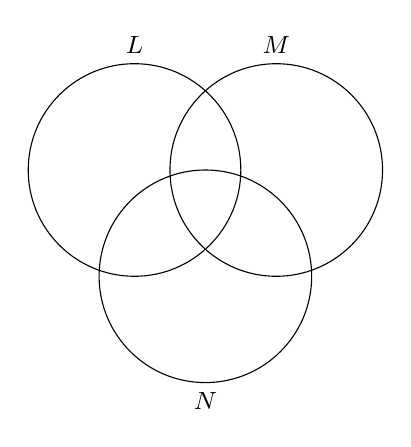
\begin{tikzpicture}[font=\small,scale=.9]
\draw (0,0)circle (1.5) (0,1.5) node[above] {$L$};
\draw(2,0) circle (1.5) (2,1.5) node [above]  {$M$};
\draw(1,-1.5)circle (1.5) (1,-3) node[below]{$N$};
\end{tikzpicture}

\end{center}
\end{esercizio}

\begin{esercizio}
 \label{ese:\thechapter.54}
Dati gli insiemi~$C$ delle lettere della parola ``GIARDINO'' e~$D$ delle lettere della
parola ``ORA'', determina la loro unione aiutandoti con la rappresentazione grafica.
 \end{esercizio}

\begin{esercizio}
\label{ese:\thechapter.55}
Determina l'unione tra i seguenti insiemi:

\begin{enumeratea}
 \item $A=\{-3$, $-2$, $-1$, $0$, $+1$, $+2$, $+3\}$, $B=\{-2$, $-1$, $0$, $+1$, $+2$, $+3$, $+4\}$. $A\cup B=\dotfill$;
 \item $A=\{x\in\insN\mid 2\le x\le 5\}$, $B=\{x\in\insN\mid 3<x<7\}$. $A\cup B=\dotfill$;
 \item $A=\{x\in\insZ\mid -5\le x\le +5\}$, $B=\{x\in\insZ\mid -15\le x<3\}$. $A\cup B=\dotfill$;
 \item $A=\{x\in\insN\mid x>100\}$, $B=\{x\in\insN\mid 10<x<20\}$. $A\cup B=\dotfill$;
 \item $A=\{l$ è una lettera di ``SATURNO''$\}$, $B=\{l$ è una lettera di ``NETTUNO''$\}$. $A\cup B=\dotfill$.
\end{enumeratea}
\end{esercizio}

\subsubsection*{\thechapter.7 - Insieme intersezione}
 \begin{esercizio}
 \label{ese:\thechapter.56}
Dati~$A=\{\text{1, 2, 4, 5}\}$ e~$B=\{\text{1, 3, 4, 5, 8}\}$ determina la loro
intersezione dopo aver rappresentato gli insiemi mediante diagrammi di
Eulero-Venn.
\end{esercizio}

\begin{esercizio}
 \label{ese:\thechapter.57}
Dati gli insiemi~$C$ delle lettere della parola ``LIBRO'' e~$D$ delle lettere della
parola ``PASTA'' determina la loro intersezione aiutandoti con la rappresentazione grafica.
\end{esercizio}

\begin{esercizio}
 \label{ese:\thechapter.58}
Considerando i~3 insiemi~$S=\{$a, b, c, e, f, s, t$\}$, $T=\{$a, c, g, h, l, s$\}$ e~$U=\{$b, c, d, g, s, t$\}$,
determina l'insieme intersezione dando sia la rappresentazione grafica sia quella tabulare.
 \end{esercizio}

\begin{esercizio}
 \label{ese:\thechapter.59}
 Determina l'intersezione tra i seguenti insiemi:
\begin{enumeratea}
 \item $A=\{-3$, $-2$, $-1$, $0$, $+1$, $+2$, $+3\}$, $B=\{-2$, $-1$, $0$, $+1$, $+2$, $+3$, $+4\}$; $A\cap B=\ldots$
 \item $A=\{x\in\insN\mid 2\le x\le~5\}$, $B=\{x\in\insN\mid 3<x<7\}$; $B\cap A=\ldots$
 \item $A=\{x\in\insZ\mid -5\le x\le+5\}$, $B=\{x\in\insZ\mid -15\le x<3\}$; $A\cap B=\ldots$
 \item $A=\{x\in\insN\mid x>100\}$, $B=\{x\in\insN\mid 10<x<20\}$; $B\cap A=\ldots$
 \item $A=\{l$ una lettera di ``SATURNO''$\}$, $B=\{l$ una lettera di ``NETTUNO''$\}$; $A\cap B=\ldots$
 \item $A=\{x\in\insQ\mid x\ge -4\}$, $B=\{x\in\insQ\mid x\le 4\}$; $A\cap B=\ldots$
\end{enumeratea}
\end{esercizio}

\subsubsection*{\thechapter.8 - Insieme differenza}
\begin{esercizio}
\label{ese:\thechapter.60}
Dati gli insiemi~$E=\{x\mid x$ è una lettera della parola ``cartellone''$\}$ e
$F=\{x\mid x$ è una lettera della parola ``martello''$\}$, determina
$E-F$ e~$F-E$.
\end{esercizio}

\begin{esercizio}
\label{ese:\thechapter.61}
Dati gli insiemi $A=\{x\in\insQ\mid 3<x\le 5\}$ e $B=\{x\in\insQ\mid x>0\}$ calcola le differenze:
\begin{multicols}{2}
\begin{enumeratea}
 \item $A-B=\ldots$
 \item $B-A=\ldots$
\end{enumeratea}
\end{multicols}
\end{esercizio}

\begin{esercizio}
\label{ese:\thechapter.62}
Determina la differenza tra i seguenti insiemi:
\begin{enumeratea}
\item $A=\{-3$, $-2$, $-1$, $0$, $+1$, $+2$, $+3\}$, $B=\{-2$, $-1$, $0$, $+1$, $+2$, $+3$, $+4\}$. $A-B=\ldots$;
\item $A=\{x\in\insN\mid 2\le x\le~5\}$, $B=\{x\in\insN\mid 3<x<7\}$. $B-A=\ldots$;
\item $A=\{x\in\insZ\mid -5\le x\le +5\}$, $B=\{x\in\insZ\mid -15\le x<3\}$. $A-B=\ldots$;
\item $A=\{x\in\insN\mid x>100\}$, $B=\{x\in\insN\mid 10<x<20\}$. $B-A=\ldots$;
\item $A=\{x\in\insN\mid 10\le x\le~100\}$ e~$B=\{y\in\insN\mid 10<y<100\}$. $A-B=\ldots$
\item $A=\{l$ è una lettera di ``SATURNO''$\}$, $B=\{l$ è una lettera di ``NETTUNO''$\}$. $A-B=\ldots$
\end{enumeratea}
\end{esercizio}

\subsubsection*{\thechapter.9 - Insieme complementare}
\begin{esercizio}
\label{ese:\thechapter.63}
Verifica, utilizzando la rappresentazione grafica, che
\begin{multicols}{2}
 \begin{enumeratea}
 \item $\overline{A}_{U}\cup A=U$;
 \item $(A-B)\cup (B-A)\cup (\overline{A\cup B})=\overline{A\cap B}$.
 \end{enumeratea}
\end{multicols}
\end{esercizio}

\begin{esercizio}
 \label{ese:\thechapter.64}
Dati~$E$ ed~$F$ sottoinsiemi di un insieme~$U$, l'insieme
definito da~$\overline{E\cap F}$ è uguale a:
\begin{center}
\boxA\quad~$E\cup F$\quad\boxB\quad~$\overline{E\cup F}$\quad\boxC\quad~$E\cap F$\quad\boxD\quad~$\overline{E}\cup\overline{F}$
\end{center}
\end{esercizio}

\begin{esercizio}
 \label{ese:\thechapter.65}
Dati~$G$ ed~$H$ sottoinsiemi di un insieme~$U$, l'insieme
definito da~$\overline{G\cup H}$ è uguale a:
\begin{center}
\boxA\quad~$\overline{G\cap H}$\quad\boxB\quad~$\overline{G}\cap\overline{H}$\quad\boxC\quad~$\overline{G\cap \overline{H}}$\quad\boxD\quad nessuno dei precedenti
\end{center}
\end{esercizio}
\pagebreak
\begin{esercizio}
\label{ese:\thechapter.66}
Dati i seguenti insiemi~$A=\{x\in\insN\mid x\le~25\}$, $B=\{x\in\insN\mid 4<x\le~9\}$, $C=\{x\in\insN\mid x<25\}$ e~$D=\{x\in\insN\mid x>7\}$.
Scegli fra i seguenti i loro complementari.
\begin{multicols}{2}
\begin{enumeratea}
\item $E=\{x\in\insN\mid x\ge~25\}$;
\item $F=\{x\in\insN\mid x\le~6\}$;
\item $G=\{x\in\insN\mid x>25\}$;
\item $H=\{x\in\insN\mid x<7\}$;
\item $I=\{x\in\insN\mid x<4\text{ e }x\ge~8\}$;
\item $L=\{x\in\insN\mid x<4\text{ o }x\ge~10\}$;
\item $M=\{x\in\insN\mid x\le~4\text{ e }x\ge~9\}$.
\end{enumeratea}
\end{multicols}
\end{esercizio}

\subsubsection*{\thechapter.10 - Leggi di De Morgan}

\begin{esercizio}
 \label{ese:\thechapter.67}
 Dimostra la seconda legge di De Morgan, annerendo gli spazi opportuni.
 \begin{center}
 %\usetikzlibrary{decorations.markings}
%\usetikzlibrary{matrix,fit}
%\usetikzlibrary{positioning}
%\usetikzlibrary{shapes.geometric}
%\usetikzlibrary{decorations.pathreplacing}
%\usetikzlibrary{decorations.text}
%\usetikzlibrary{mindmap}
%\usetikzlibrary{plotmarks}
%\usetikzlibrary{backgrounds}
%\usetikzlibrary{patterns}

% (c) 2012 Dimitrios Vrettos - d.vrettos@gmail.com

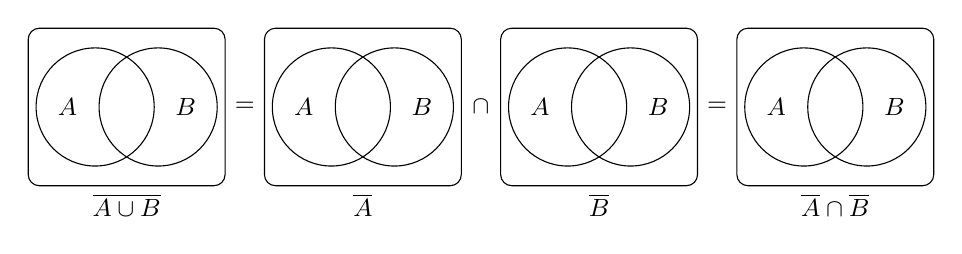
\begin{tikzpicture}[x=5mm,y=5mm,font=\small, outline/.style={draw=circle edge}]
\definecolor{circle area}{gray}{0.9}
\definecolor{circle edge}{rgb}{0,0,0}

\def\firstcircle{(1.7,2) circle (1.5)}
\def\secondcircle{(3.3,2) circle (1.5)}

\begin{scope}[rounded corners]
\foreach \i in {0,6,12,18}
\draw[fill=white] (\i,0) rectangle (\i+5,4);
\end{scope}

\begin{scope}]
\begin{scope}
\clip \firstcircle;
\fill[white] \secondcircle;
\end{scope}
\draw[outline] \firstcircle;
\draw[outline] \secondcircle;
\end{scope}

\begin{scope}[xshift=30mm]
\begin{scope}
\clip \firstcircle;
\fill[white] \firstcircle;
\end{scope}
 \draw[outline]  \firstcircle;
\draw[outline] \secondcircle;
\end{scope}

\begin{scope}[xshift=60mm]
\begin{scope}
\clip \secondcircle;
\fill[white] \secondcircle;
\end{scope}
 \draw[outline]  \firstcircle;
\draw[outline] \secondcircle;
\end{scope}

\begin{scope}[xshift=90mm]
\begin{scope}
\clip \firstcircle;
\fill[white] \secondcircle;
\end{scope}
\draw[outline] \firstcircle;
 \draw[outline] \secondcircle;
\end{scope}

\foreach \x/\xtext in {5.5/$=$,11.5/$\cap$,17.5/$=$}
	\node  at (\x,2) {\xtext};

\foreach \y in {1,7,13,19}
\node  at (\y,2) {$A$};

\foreach \z in {4,10,16,22}
\node  at (\z,2) {$B$};

\foreach \j/\jtext in {2.5/\overline{A\cup B},8.5/\overline{A},14.5/\overline{B},20.5/\overline{A}\cap\overline{B}
}
\node  at (\j,-.5) {$\jtext$};
\end{tikzpicture}



 \end{center}
\end{esercizio}

\subsubsection*{\thechapter.11 - Partizione di un insieme}

\begin{esercizio}
\label{ese:\thechapter.68}
Dato~$A=\{\text{do, re, mi}\}$ determina l'insieme delle parti~$\wp (A)$.
\end{esercizio}

\begin{esercizio}
 \label{ese:\thechapter.69}
 Determina una partizione dell'insieme~$L$ delle lettere dell'alfabeto.
\end{esercizio}

\begin{esercizio}
 \label{ese:\thechapter.70}
 Fai un esempio di partizione possibile dei libri di una biblioteca.
\end{esercizio}

\begin{esercizio}
 \label{ese:\thechapter.71}
 Dai un esempio di partizione dell'insieme dei triangoli.
\end{esercizio}

\subsubsection*{\thechapter.12 - Prodotto cartesiano fra insiemi}

\begin{esercizio} %modificato da Antonio
\label{ese:\thechapter.72}
Sia~$E=\{x\in\insN\mid 1\le x<3\}$, $F=\{x\mid x$ è una vocale della parola ``TELEFONO''$\}$ e~$G=\{x\in\insN\mid x<-6\}$, calcola $E\times F$,  $F\times E$,  $F\times G$,  $G\times E$.
\end{esercizio}

\begin{esercizio} %modificato da Antonio
 \label{ese:\thechapter.73}
Quanti sono gli elementi del prodotto cartesiano~$A\times B$, dove~$A$ ha~6 elementi, $B$ ne ha~3?
\end{esercizio}


\begin{esercizio} %modificato da Antonio
 \label{ese:\thechapter.74}
Sapendo che~$E\times F=\{(\text{x};\text{x})\text{, }(\text{x};\text{y})\text{, }(\text{x};\text{z})\text{, }(\text{y};\text{x})\text{, }(\text{y};\text{y})\text{, }(\text{y};\text{z})\}$, indica gli elementi di~$E$ e di~$F$.
\end{esercizio}

\begin{esercizio} %modificato da Antonio
 \label{ese:\thechapter.75}
Se~$A\times B$ ha~5 elementi, da quanti elementi possono essere costituiti~$A$ e~$B$?
\end{esercizio}

\begin{esercizio}
 \label{ese:\thechapter.76}
Dati gli insiemi~$A=\{\text{3, 5, 6}\}$ e~$B=\{-2\text{, }1\}$ costruisci il
diagramma cartesiano di~$A\times B$ ed elencane gli elementi.
\end{esercizio}

\begin{esercizio}
 \label{ese:\thechapter.77}
 Dato~$A=\{\text{0, 1, 2}\}$ calcola~$A\times A$.
\end{esercizio}

\subsubsection*{\thechapter.13 - I diagrammi di Eulero-Venn come modello di un problema}

\begin{esercizio}[\Ast]
\label{ese:\thechapter.78}
La scuola ``Step'' organizza corsi di Salsa, Hip Hop e Break Dance.

\begin{enumeratea}
\item Gli iscritti ai corsi sono in tutto~98;
\item 6 frequentano tutti e tre i corsi;
\item 37 frequentano il corso di Salsa;
\item 15 solo i corsi di Salsa e di Hip Hop;
\item 7 solo i corsi Salsa e Break Dance;
\item 9 almeno Hip Hop e Break Dance;
\item 28 Salsa o Break Dance ma non Hip Hop.
\end{enumeratea}

Quanti praticano solo Hip Hop?

Rappresentiamo la situazione con un diagramma di Eulero-Venn.
\begin{center}
 % (c) 2012 Dimitrios Vrettos - d.vrettos@gmail.com
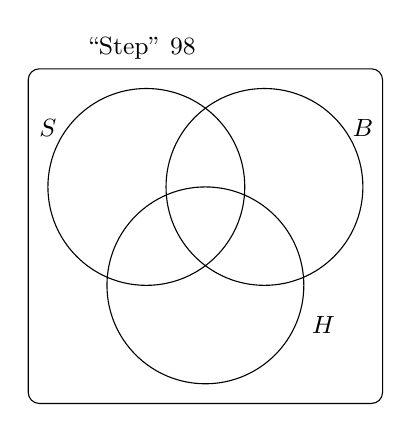
\begin{tikzpicture}[x=5mm, y=5mm,font=\small]

\draw[rounded corners] (0,-5.5) rectangle (9,3) (4.5,3)node[above, anchor=south east] {``Step'' 98};

\draw(3,0) circle (2.5);
\draw(6,0) circle (2.5);
\draw(4.5,-2.5) circle (2.5);

\node at (.5,1.5) {$S$};
\node at (8.5,1.5) {$B$};
\node at (7.5,-3.5) {$H$};

\end{tikzpicture}

\end{center}
$S$ è l'insieme degli iscritti al corso di Salsa, $B$ l'insieme degli iscritti al corso di
Break Dance, $H$ l'insieme degli iscritti al corso di Hip Hop.
\end{esercizio}

\begin{esercizio}
\label{ese:\thechapter.79}
Il club ``Argento vivo'' ha~$\np{2500}$ iscritti; nel mese di gennaio ha organizzato alcune
manifestazioni sportive alle quali hanno partecipato~850 degli iscritti
e alcuni tornei di scacchi ai quali hanno partecipato in~780. 320
iscritti al club hanno potuto partecipare, grazie alla perfetta
organizzazione, sia alle manifestazioni sportive sia ai tornei di
scacchi. Quanti soci del club non hanno partecipato a nessuna delle
iniziative e quanti invece hanno partecipato ad almeno una?
\end{esercizio}

\begin{esercizio}[\Ast]
 \label{ese:\thechapter.80}
In una scuola di musica si tengono~4 corsi di cui quello di pianoforte è obbligatorio
per tutti i~100 studenti iscritti, mentre quelli di violino, flauto e
chitarra sono facoltativi. Per essere ammessi agli esami di fine anno
bisogna frequentare almeno un corso oltre a quello di pianoforte. Se gli alunni:

\begin{enumeratea}
 \item che frequentano il corso di flauto sono~25 e non frequentano né quello di violino, né quello di chitarra;
 \item iscritti sia al corso di violino sia a quello di chitarra sono~20;
 \item che frequentano il corso di violino sono~46;
 \item che frequentano solo il corso di violino sono tanti quanti quelli che frequentano solo il corso di chitarra.
\end{enumeratea}

Quanti alunni non possono sostenere l'esame finale?
Quale dei seguenti diagrammi di Eulero-Venn può essere preso come modello della situazione?
\begin{center}
 % (c) 2012 Dimitrios Vrettos - d.vrettos@gmail.com
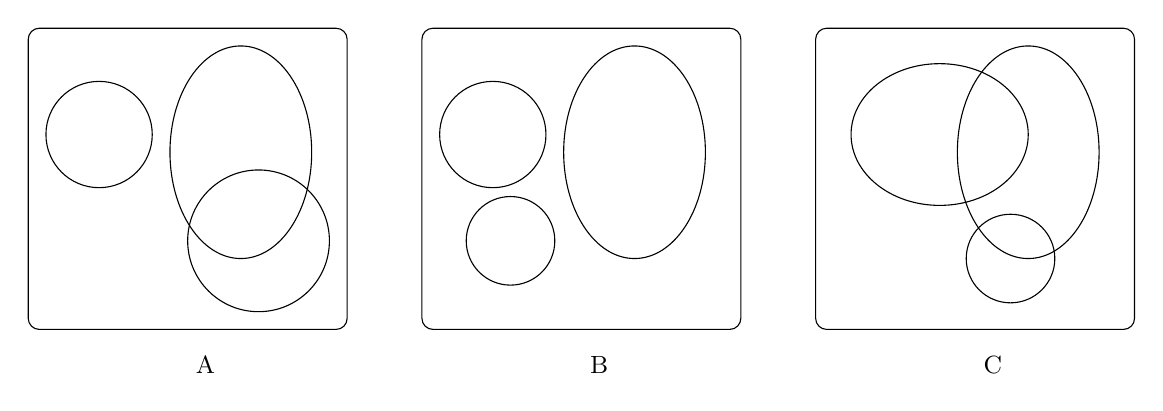
\begin{tikzpicture}[x=4.5mm, y=4.5mm,font=\small]

\draw[rounded corners] (0,-5.5) rectangle (9,3) (5,-6)node[below] {A};
\draw(2,0) circle (1.5);
\draw (6,-.5)ellipse (2 and 3);
\draw(6.5,-3) circle (2);

\begin{scope}[xshift=50mm]
\draw[rounded corners] (0,-5.5) rectangle (9,3) (5,-6)node[below] {B};
\draw(2,0) circle (1.5);
\draw (6,-.5)ellipse (2 and 3);
\draw(2.5,-3) circle (1.25);
\end{scope}

\begin{scope}[xshift=100mm]
\draw[rounded corners] (0,-5.5) rectangle (9,3) (5,-6)node[below] {C};
\draw(3.5,0) ellipse (2.5 and 2);
\draw (6,-.5)ellipse (2 and 3);
\draw(5.5,-3.5) circle (1.25);
\end{scope}
\end{tikzpicture}

\end{center}

\end{esercizio}
\begin{multicols}{2}
\begin{esercizio}[\Ast]
\label{ese:\thechapter.81}
I componenti di una compagnia teatrale sanno almeno cantare, ballare,
recitare. Al termine di una rappresentazione si sa che~12 hanno almeno
ballato, 8 hanno almeno cantato e~16 hanno almeno recitato. La
versatilità dei componenti ha permesso che~5 abbiano almeno ballato e
cantato, 3 abbiano almeno cantato e recitato, 8 abbiano almeno ballato e
recitato, 2 ballerini hanno ballato, cantato e recitato. Quanti sono i
componenti della compagnia?
\end{esercizio}

\begin{esercizio}[\Ast]
\label{ese:\thechapter.82}
Da un'indagine condotta su consumatori adulti è
risultato che~605 bevono almeno vino, 582 bevono almeno latte, 348
bevono almeno birra, 140 bevono almeno vino e birra, 85 bevono almeno
vino e latte, 56 bevono almeno latte e birra, 25 bevono tutte e tre le
bevande mentre~71 non bevono alcuna delle bevande citate.
\begin{enumeratea}
\item Quante persone bevono una sola bevanda?
\item quante bevono almeno una bevanda?
\item quante sono le persone intervistate?
\end{enumeratea}
\end{esercizio}

\begin{esercizio}[\Ast]
\label{ese:\thechapter.83}
In una scuola di lingue sono iscritti~164 studenti; 80 seguono il
corso di francese e~120 il corso di tedesco. Quanti studenti seguono
entrambi i corsi? Quanti studenti seguono
solo il corso di tedesco?
\end{esercizio}

\begin{esercizio}
\label{ese:\thechapter.84}
In un classe di~28 allievi, 18 frequentano il laboratorio di teatro,
22 il laboratorio di fotografia, 3 non frequentano alcun laboratorio.
Rappresenta la situazione con un diagramma di Eulero-Venn. Quanti
allievi frequentano entrambi i laboratori? Quanti frequentano almeno un
laboratorio? Quanti non frequentano il laboratorio di teatro?
\end{esercizio}

\begin{esercizio}
\label{ese:\thechapter.85}
In una pizzeria, domenica sera, erano presenti~140 persone: 50 hanno
mangiato pizza e calzone, 20 hanno mangiato solo calzone e~15 non hanno
mangiato né pizza né calzone. Il pizzaiolo si chiede se può
conoscere in base alle precedenti informazioni, quante pizze ha
preparato. Aiutalo a risolvere il suo problema illustrando la
situazione con un diagramma di Eulero-Venn, assegnando a ciascun insieme la
sua cardinalità.
\end{esercizio}

\begin{esercizio}
\label{ese:\thechapter.86}
In un paese di~$\np{3200}$ abitanti arrivano due quotidiani: il primo è letto da~850
persone, il secondo da~780. Poiché~320 persone leggono entrambi i
quotidiani, quante persone non leggono alcun quotidiano e quante almeno uno?
\end{esercizio}

\begin{esercizio}[Test di ammissione ad Architettura~2008]
\label{ese:\thechapter.87}
Nella classe di Asdrubale ci sono~37 allievi. Tutti si sono iscritti
ad almeno una delle due attività extracurriculari (musica e
pallavolo). Alla fine~15 fanno musica e~28 fanno pallavolo.
Quanti allievi, frequentando entrambe le attività, hanno la
necessità di programmare gli orari per evitare sovrapposizioni?
\begin{center}
 \boxA~13\quad\boxB~9\quad\boxC~16\quad\boxD~22\quad\boxE~6
\end{center}
\end{esercizio}

\begin{esercizio}[Test di ammissione a Medicina~2008]
\label{ese:\thechapter.88}
In un'aula scolastica, durante la ricreazione, 14
studenti stanno seduti, 8 mangiano la pizza. Con questi dati si può
concludere con certezza che il numero totale~$N$ degli studenti è:
\begin{center}
 \boxA\quad~$N>14$\quad\boxB\quad~$N<14$\quad\boxC\quad~$N>22$\quad\boxD\quad~$N = 22$\quad\boxE\quad~$N\ge~14$
\end{center}
\end{esercizio}

\begin{esercizio}
\label{ese:\thechapter.89}
In una scuola di~150 alunni ci sono~23 studenti che frequentano il corso ECDL, 41 studenti che frequentano solo il corso di Inglese, 3
studenti che frequentano tutti e due i corsi. Quanti sono gli studenti che frequentano solo il corso ECDL? Quanti studenti non frequentano
nessuno dei due corsi?
\end{esercizio}

\begin{esercizio}
\label{ese:\thechapter.90}
In un giorno di vacanza, 20 alunni dovrebbero studiare latino e
matematica per recuperare le lacune: 8 non studiano latino, 10 studiano
matematica e~4 non studiano niente. Quanti alunni studiano entrambe le
materie?
\end{esercizio}

\begin{esercizio}
\label{ese:\thechapter.91}
In una classe di~20 alunni si sta organizzando una gita
scolastica. Durante l'assemblea gli alunni raccolgono
informazioni sulle mete già visitate: 18 hanno visitato Venezia, 14
Roma, 5 Firenze. Solo~3 hanno visitato tutte e tre le città, 5 hanno
visitato Firenze e Venezia, 3 solo Venezia. Quanti hanno visitato solo
Firenze? Quanti hanno visitato Firenze e Roma? Quanti non hanno
visitato nessuna delle tre città? Quanti non hanno visitato Roma?
\end{esercizio}
\end{multicols}
\subsection{Esercizi riepilogativi}

\begin{esercizio}
\label{ese:\thechapter.92}
Siano~$A=\{x\in\insN\mid 1\le x\le~15\}$ e~$B=\{x\in\insN\mid 2\le x\le 20\}$.
\begin{center}
% (c) 2012 Dimitrios Vrettos - d.vrettos@gmail.com
\begin{tikzpicture}[x=3mm, y=5mm,font=\small]

\draw[->, thick] (-1,0)--(24,0) node [above left] {$\insN$};
\draw[pattern =north east lines, pattern color=RedOrange] (1,0) rectangle (15,1) (1,1)node[left] {$A$};
\draw[pattern =north west lines, pattern color=CornflowerBlue] (2,0) rectangle (20,1.5) node[right]{$B$};

\foreach \x/\xtext in {1/1,2/2,15/15,20/20}
\draw[fill] (\x,0)circle (1pt) (\x,0)node [below]{\xtext};
\end{tikzpicture}

\end{center}
Quale delle seguenti affermazioni è vera:
\begin{center}
\boxA\quad~$A\subset B$\quad\boxB\quad~$B\supset A$\quad\boxC\quad$A=B$\quad\boxD\quad$B\not\subset A$
\end{center}
\end{esercizio}

\begin{esercizio}
\label{ese:\thechapter.93}
 Siano~$A=\{x\in\insN\mid x$ è pari e $(1\le x\le 20)\}$ e~$B=\{x\in\insN\mid x$ è multiplo di~6 e $2\le x\le 18\}$.
Quale affermazione è vera?
\begin{center}
 \boxA\quad~$A\subset B$\quad\boxB\quad~$B\supset A$\quad\boxC\quad~$A=B$\quad\boxD\quad~$B\subset A$
\end{center}
\end{esercizio}

\begin{esercizio}
\label{ese:\thechapter.94}
Siano~$A=\{x\in\insN\mid 3\le x\le 10\}$ e~$B=\{x\in\insN\mid 2\le x\le 20\}$.
Quali delle seguenti affermazioni è vera:
\begin{center}
 \boxA\quad~$A\subset B$\quad\boxB\quad~$B\supset A$\quad\boxC\quad~$A=B$\quad\boxD\quad~$B\not\subset A$
\end{center}
\end{esercizio}

\begin{esercizio}
\label{ese:\thechapter.95}
Individua tutti i possibili sottoinsiemi propri formati da tre elementi dell'insieme~$C=\{$a, e, i, o, u$\}$.
\end{esercizio}

\begin{esercizio}
\label{ese:\thechapter.96}
Sia~$A=\{$1, 2, 3, 4$\}$ scrivi i possibili sottoinsiemi propri e impropri di~$A$.
\end{esercizio}
\pagebreak
\begin{esercizio}
\label{ese:\thechapter.97}
Associa a ogni diagramma la corretta rappresentazione grafica (ci può essere più di una risposta corretta).

\TabPositions{5cm}
\begin{enumeratea}
 \item $M\subset P$ \tab\boxA\quad\boxB\quad\boxC\quad\boxD\quad\boxE
\item $P\supseteq M$ \tab\boxA\quad\boxB\quad\boxC\quad\boxD\quad\boxE
\item $M\subseteq (M\cup P)$ \tab\boxA\quad\boxB\quad\boxC\quad\boxD\quad\boxE
\item $M\not\subset P$ \tab\boxA\quad\boxB\quad\boxC\quad\boxD\quad\boxE
\item $P\subset (P\cup M)$ \tab\boxA\quad\boxB\quad\boxC\quad\boxD\quad\boxE
\item $M\neq P$ \tab\boxA\quad\boxB\quad\boxC\quad\boxD\quad\boxE
\end{enumeratea}
\begin{center}
% (c) 2012 Dimitrios Vrettos - d.vrettos@gmail.com
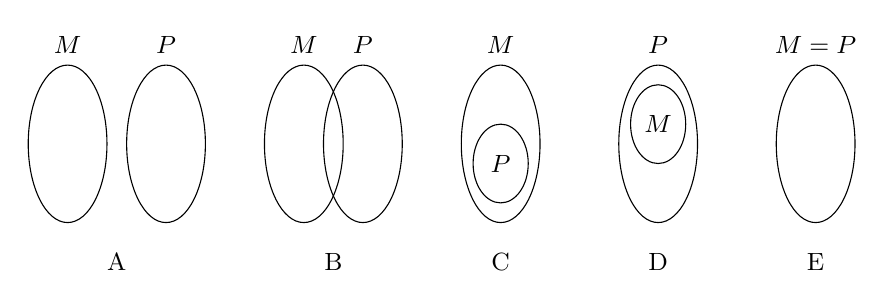
\begin{tikzpicture}[x=5mm, y=5mm,font=\small]

\draw (0,0) ellipse (1 and 2) (0,2.5)node {$M$};
\draw (2.5,0) ellipse (1 and 2)(2.5,2.5) node {$P$};
\node  at (1.25,-3) {A};

\begin{scope}[xshift=30mm]
\draw (0,0) ellipse (1 and 2) (0,2.5)node {$M$};
\draw (1.5,0) ellipse (1 and 2)(1.5,2.5) node {$P$};
\node  at (.75,-3) {B};
\end{scope}

\begin{scope}[xshift=55mm]
\draw (0,0) ellipse (1 and 2) (0,2.5)node {$M$};
\draw (0,-.5) ellipse (.7 and 1) node {$P$};
\node  at (0,-3) {C};
\end{scope}

\begin{scope}[xshift=75mm]
\draw (0,0) ellipse (1 and 2) (0,2.5)node {$P$};
\draw (0,.5) ellipse (.7 and 1) node {$M$};
\node  at (0,-3) {D};
\end{scope}

\begin{scope}[xshift=95mm]
\draw (0,0) ellipse (1 and 2) (0,2.5)node {$M=P$};
\node  at (0,-3) {E};
\end{scope}
\end{tikzpicture}

\end{center}
\end{esercizio}

\begin{esercizio}
\label{ese:\thechapter.98}
Dati $A=\{$2, 4, 6, 8, 10, 12, 14, 16, 18, 20$\}$, $B=\{$3, 6, 9, 12, 15, 18$\}$ e
$C=\{$1, 3, 5, 7, 9, 11, 13, 15, 17, 19$\}$, calcola
$A\cap B$, $A\cup C$, $(A\cap B)\cup C$, $B\cap C$, $(A\cup B)\cap(B\cup C)$.
\end{esercizio}

\begin{esercizio}
\label{ese:\thechapter.99}
Sia $M=\{l$ una lettera di ``MATEMATICA''$\}$, $A=\{l$ una lettera di ``ALGEBRA''$\}$, $G=\{l$ una lettera di ``GEOMETRIA''$\}$, $I=\{l$ una lettera di ``INFORMATICA''$\}$ calcola:
\begin{multicols}{3}
\begin{enumeratea}
 \item $M\cup A$;
 \item $A\cup G$;
 \item $A\cap I$;
 \item $M\cap G$;
 \item $M\cup A \cup G \cup I$;
 \item $M\cap A \cap G \cap I$;
 \item $M\cup (A\cap G)$;
 \item $M\cap (G\cup I)$;
 \item $M-A$;
 \item $A-G$;
 \item $I-(A\cup B)$;
 \item $(A\cup B)-(M\cap I)$.
\end{enumeratea}
\end{multicols}
\end{esercizio}

\begin{esercizio}
\label{ese:\thechapter.100}
Sia~$M_{3}$ l'insieme dei multipli~3 e~$M_{4}$ l'insieme dei multipli di~4, in
generale~$M_{n}$ l'insieme dei multipli del numero~$n$.

 \begin{enumeratea}
 \item Calcola~$M_{3}\cap M_{4}$. Si tratta di~$M\ldots$ l'insieme dei multipli di \ldots;
 \item calcola~$M_{6}\cap M_{4}$. Si tratta di~$M\ldots$ l'insieme dei multipli di \ldots;
 \item calcola~$M_{60}\cap M_{48}$ \ldots;
 \item sai dedurre una regola che, dati due numeri naturali~$m$ e~$n$ calcoli~$M_{m}\cap M_{n}$? Può accadere che questo insieme sia vuoto?
 \end{enumeratea}
\end{esercizio}

\begin{esercizio}
\label{ese:\thechapter.101}
Sia~$D_{4}$ l'insieme dei divisori di~4 e~$D_{6}$ l'insieme dei divisori di~6, in
generale~$D_{n}$ l'insieme dei divisori del numero~$n$.

\begin{enumeratea}
 \item Calcola~$D_{4}\cap D_{6}$. Si tratta di~$D\ldots$ l'insieme dei divisori di \ldots;
 \item calcola~$D_{60}\cap D_{48}$ \ldots;
 \item sai dedurre una regola che, dati due numeri naturali~$m$ e~$n$,
calcoli~$D_{m}\cap D_{n}$? Può accadere che questo insieme sia
vuoto? Qual è il numero minimo di elementi che può contenere?
\end{enumeratea}
\end{esercizio}
\pagebreak
\begin{esercizio} %Modificato da Antonio
\label{ese:\thechapter.102}
Determina l'insieme intersezione~$A\cap B$ e l'insieme unione~$A\cup B$.
\begin{enumeratea}
 \item $A=\{x\mid x\in\insQ,0<x<\frac{3}{2}\}$ e~$B=\{x\mid x\in\insQ\text{, }1<x<6\}$;
 \item $A=\{x\mid x\in\insQ,-1<x<0\}$ e~$B=\{x\mid x\in\insQ\text{, }\frac{1}{3}<x<6\}$;
 \item $A=\{x\mid x\in\insQ,-5<x<10\}$ e~$B=\{x\mid x\in\insQ\text{, }\frac{1}{3}<x<6\}$;
 \item $A=\{x\mid x\in\insQ,0\le x<10\}$ e~$B=\{x\mid x\in\insQ\text{, }\frac{1}{3}<x\le~6\}$.
 \item $M\cup A \cup G \cup I$;
 \item $M\cap A \cap G \cap I$;
 \item $M\cup (A\cap G)$;
 \item $M\cap (G\cup I)$;
 \item $M-A$;
 \item $A-G$;
 \item $I-(A\cup B)$;
 \item $(A\cup B)-(M\cap I)$.
\end{enumeratea}
\end{esercizio}

\begin{esercizio}
\label{ese:\thechapter.103}
Dato l'insieme~$A=\{$3, 4, 5, 6, 7, 8, 9, 12, 32$\}$ e il suo sottoinsieme~$B$ dei multipli di~3, determina gli
insiemi~$A-B$ e~$B-A$.
\end{esercizio}

\begin{esercizio}
\label{ese:\thechapter.104}
Dati gli insiemi~$C$ e~$D$ tali che~$C\subset D$
completa le seguenti relazioni aiutandoti con la rappresentazione
grafica:
\begin{multicols}{3}
\begin{enumeratea}
\item $D-C=\ldots$;
\item $D\cap \overline{C}=\ldots$;
\item $\overline{C\cap D}=\ldots$;
\item $C\cup \overline{C}=\ldots$;
\item $C-D=\ldots$;
\item $C\cap \overline{C}=\ldots$
\end{enumeratea}
\end{multicols}
\end{esercizio}

\begin{esercizio}
\label{ese:\thechapter.105}
Quale delle seguenti scritture corrisponde a~$\overline{{X\cap \overline{Y}}}$:
\begin{multicols}{4}
 \begin{enumeratea}
 \item $\overline{X}\cup \overline{Y}$
 \item $\overline{X}\cap \overline{Y}$
 \item $\overline{X}\cup Y$
 \item $X\cup \overline{Y}$
 \end{enumeratea}
\end{multicols}
\end{esercizio}

\begin{esercizio}
\label{ese:\thechapter.106}
Esegui le operazioni~$A\cup B$, $A\cap B$, $A-B$ tra i seguenti insiemi.

\begin{enumeratea}
\item $A=\{$2, 4, 6, 8$\}$, $B=\{$1, 3, 6, 9$\}$;
\item $A=\{$a, e, i, o, u$\}$, $B=\{$a, b, c, d, e$\}$;
\item $A=\{x\in\insN\mid x$ è lettera di ``casa''$\}$, $B=\{x\in\insN\mid x$ è lettera di ``caserma''$\}$;
\item $A=\{x\in\insN\mid x$ è pari$\}$, $B=\{x\in\insN\mid x$ è dispari$\}$;
\item $A=\{x\in\insN\mid x$ è multiplo di~2$\}$, $B=\{x\in\insN\mid x$ è multiplo di~4$\}$;
\item $A=\{x\in\insZ\mid -5\le x\le~5\}$, $B=\{x\in\insZ\mid -2\le x\le~8\}$;
\item $A=\emptyset$, $B=\{0\}$.
\end{enumeratea}
\end{esercizio}

\begin{esercizio}
\label{ese:\thechapter.107}
Sia $A=\{a$ una lettera di ``MATEMATICA''$\}$, $B=\{b$ una lettera di ``FILOSOFIA''$\}$, $C=\{c$ una lettera di ``GEOMETRIA''$\}$, $D=\{d$ una lettera di ``ITALIANO''$\}$ calcola:
\begin{multicols}{3}
\begin{enumeratea}
 \item $A\cap B$;
 \item $A\cap C$;
 \item $A\cap D$;
 \item $A\cap B \cap C \cap D$;
 \item $A\cup B \cup C \cap D$;
 \item $A\cup (B\cap C)$;
 \item $B\cap (A\cup C)$;
 \item $A-D$;
 \item $D-A$.
\end{enumeratea}
\end{multicols}
\end{esercizio}

\begin{esercizio}
\label{ese:\thechapter.108}
Dati gli insiemi $U=\{\text{0, 1, 2, 3, 4, 5, 6, 7, 8, 9} \}$, $A=\{\text{0, 1, 2, 3, 4, 5}\}$, $B=\{\text{4, 5, 6, 7, 8, 9}\}$, $C=\{\text{3, 4, 5, 6, 7, 8}\}$, dire se $A$, $B$, $C$ sono equipotenti, se i tre insiemi costituiscono una partizione di~$U$ e scrivere per elencazione gli insiemi risultanti dalle seguenti operazioni:
\begin{multicols}{3}
\begin{enumeratea}
 \item $A\cap B$;
 \item $B\cap C$;
 \item $B\cup C$;
 \item $A\cup B$;
 \item $A\cup B \cup C$;
 \item $A\cap B\cap C$.
\end{enumeratea}
\end{multicols}
\end{esercizio}

\begin{esercizio}
\label{ese:\thechapter.109}
Dato~$A=\{x\in\insN\mid x$ è multiplo di~2$\}$ determina~$\complement_{\insN}A$.
\end{esercizio}

\begin{esercizio}
\label{ese:\thechapter.110}
Dato~$A=\{$I, II, III$\}$ e~$B=\{$a, b$\}$ determina~$A\times B$.
\end{esercizio}

\begin{esercizio}
\label{ese:\thechapter.111}
Dato~$B=\{\text{1, 2, 3}\}$ calcola~$(B\cup B)\cap B$.
\end{esercizio}

\begin{esercizio}
\label{ese:\thechapter.112}
Dati $A=\{x\in\insZ\mid -5\le x<2\}$ e $B=\{x\in\insN\mid -3<x\le~2\}$, calcola
$A\cup B$, $A\cap B$, $B-A$, $\complement_{A}B$, $A\times(A\cap B)$ e~$\wp (B-A)$.
\end{esercizio}

\begin{esercizio}
\label{ese:\thechapter.113}
Per ciascuna delle seguenti affermazioni false dai un controesempio.

\begin{enumeratea}
\item $A\cup B=A$;
\item $A\cap B=\emptyset\:\Rightarrow\:A=\emptyset $;
\item se~$x$ è multiplo di~2 allora è anche multiplo di~4;
\item se~$\card A =2$ e~$\card B = 5$ allora~$\card A\cup B=7$;
\item se~$\card A =2$ e~$\card B = 5$ allora~$\card A\cap B=2$.
\end{enumeratea}
\end{esercizio}

\begin{esercizio}
\label{ese:\thechapter.114}
In base alla figura rispondi alle domande:
\begin{multicols}{2}
\TabPositions{4.5cm}
\begin{enumeratea}
\item L'insieme~$E$ ha~5 elementi \tab\boxV\quad\boxF
\item $2\in E$ \tab\boxV\quad\boxF
\item $3\notin G$ \tab\boxV\quad\boxF
\item $F\subset G$ \tab\boxV\quad\boxF
\item $F\subset E$ \tab\boxV\quad\boxF
\item $\emptyset \subseteq G$ \tab\boxV\quad\boxF
\item $\card(E)=8$ \tab\boxV\quad\boxF
\item $10\in E$ \tab\boxV\quad\boxF
\item $F\cap E=F$ \tab\boxV\quad\boxF
\item $F\cup G=E$ \tab\boxV\quad\boxF
\item $(E-F)-G=\{\text{1, 4}\}$ \tab\boxV\quad\boxF
\end{enumeratea}
\begin{center}
 % (c) 2012 Dimitrios Vrettos - d.vrettos@gmail.com
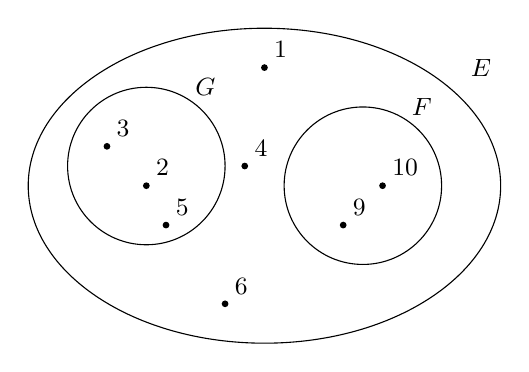
\begin{tikzpicture}[x=5mm, y=5mm,font=\small]

\draw (0,0) ellipse (6 and 4) (5.5,3)node {$E$};
\draw (2.5,0) circle (2)(4,2) node {$F$};
\draw (-3,.5) circle (2)(-1.5,2.5) node {$G$};

\draw[fill](-3,0) circle (1pt ) node[above right]  {2};
\draw[fill](-2.5,-1) circle (1pt ) node[above right]  {5};
\draw[fill](-4,1) circle (1pt ) node[above right]  {3};

\draw[fill](3,0) circle (1pt ) node[above right]  {10};
\draw[fill](2,-1) circle (1pt ) node[above right]  {9};

\draw[fill](0,3) circle (1pt ) node[above right]  {1};
\draw[fill](-.5,.5) circle (1pt ) node[above right]  {4};
\draw[fill](-1,-3) circle (1pt ) node[above right]  {6};
\end{tikzpicture}

\end{center}
\end{multicols}
\end{esercizio}

\begin{esercizio}
\label{ese:\thechapter.115}
Completa la seguente tabella:

\begin{tabular*}{.9\textwidth}{@{\extracolsep{\fill}}*{2}{cl}}
\toprule
Simbologia & Significato\\
\midrule
$A=\{a\text{, }b\text{, }c\text{, }d\}$ & $A$ è formato dagli \dotfill~$a\text{, }b\text{, }c\text{, }d$.\\
$a\in A$ & L'elemento~$a$ \dotfill all'insieme~$A$.\\
\dotfill & L'elemento f non appartiene all'insieme~$A$.\\
$B\subset A$ & L'insieme~$B$ è \ldots\ldots nell'insieme~$A$, ovvero~$B$ è un \ldots\ldots di~$A$.\\
\dotfill & L'insieme vuoto è un sottoinsieme di~$A$.\\
\dotfill & L'insieme~$C$ è l'unione degli insiemi~$A$ e~$B$.\\
$D=A\cap B$ & L'insieme~$D$ è \dotfill degli insiemi~$A$ e~$B$.\\
$A\cap F=\emptyset $& $A$ e~$F$ sono insiemi \dotfill cioè non hanno \dotfill \\
$L=\complement_{A}B$ & L'insieme~$L$ è \dotfill \\
\dotfill & L'insieme~$M$ è la differenza tra~$A$ e~$B$.\\
\bottomrule
\end{tabular*}
\end{esercizio}

\begin{esercizio}
\label{ese:\thechapter.116}
Rappresenta graficamente l'insieme~$A=\{x\in\insN\mid x\le 25$ e $x$ è pari$\}$ e
$B=\{x\in\insN\mid x\le 27$ e $x$ è multiplo di~4$\}$ e stabilisci se~$A\supseteq B$.
\end{esercizio}

\begin{esercizio}
\label{ese:\thechapter.117}
Verifica usando i diagrammi di Eulero-Venn che se~$A\subset B$ e~$B\subset C$ allora~$A\subset C$. Le relazioni valgono
anche se il simbolo~``${\subset}''$ viene sostituito con~``${\subseteq}''$?
\end{esercizio}

\begin{esercizio}
\label{ese:\thechapter.118}
Considerato l'insieme~$X=\{\text{a, c, d, t, o}\}$ stabilisci se le seguenti affermazioni sono vere o false.

\TabPositions{8cm}
\begin{enumeratea}
\item $\{x\mid x\text{ è una vocale della parola ``carota''}\} \subset X$ \tab\boxV\quad\boxF
\item $\{\text{a, t}\}\not\subset \wp (X)$ \tab\boxV\quad\boxF
\item $\{\text{a, t}\}\in \wp (X)$ \tab\boxV\quad\boxF
\item $0\in X$ \tab\boxV\quad\boxF
\item $\emptyset \in \wp (X)$ \tab\boxV\quad\boxF
\item $X\in \wp (X)$ \tab\boxV\quad\boxF
\end{enumeratea}
\end{esercizio}

\begin{esercizio}
\label{ese:\thechapter.119}
Se~$U$ è l'insieme universo degli italiani, $D$ l'insieme delle donne italiane,
$L$ l'insieme degli italiani laureati, $S$ l'insieme degli italiani sposati, cosa rappresentano
i seguenti insiemi?
\begin{multicols}{3}
\begin{enumeratea}
\item $\overline{D}$;
\item $L\cap D$;
\item $\overline{{L\cup D\cup S}}$;
\item $L-S$;
\item $\overline{{L}}\cap S$;
\item $\overline{{L\cap D\cap S}}$.
\end{enumeratea}
\end{multicols}
\end{esercizio}

\begin{esercizio}
\label{ese:\thechapter.120}
Quanti elementi ha~$\wp (H)$ sapendo che $H$ ha~7 elementi?
\end{esercizio}

\begin{esercizio}
\label{ese:\thechapter.121}
Scrivi l'insieme che ha per insieme delle parti:
$\{\emptyset\text{, }\{\text{Mauro}\}\text{, }\{\text{Mario}\}\text{, }\{\text{Mauro, Mario}\}\}$.
\end{esercizio}

\begin{esercizio}
\label{ese:\thechapter.122}
Se~$A\cup B=B$ cosa puoi dire di~$A$ e~$B$?
\begin{center}
 \boxA\quad~$B\subseteq A$\quad\boxB\quad~$A\notin B$\quad\boxC\quad~$A\subseteq B$\quad\boxD\quad~$A\subset B$\quad\boxE\quad$A\cap B=\emptyset $
\end{center}
\end{esercizio}

\begin{esercizio}
\label{ese:\thechapter.123}
Dati gli insiemi~$A=\{\text{10, 20, 30, 40, 50}\}$ e $B=\{\text{20, 30, 50}\}$,
determina un insieme~$C$ tale che:
\begin{multicols}{4}
\begin{enumeratea}
 \item $B\cup C=A$;
 \item $A\cap C=B$;
 \item $C\cup C=B$;
 \item $C\cap C=A$.
\end{enumeratea}
\end{multicols}
\end{esercizio}

\begin{esercizio}
\label{ese:\thechapter.124}
Dati gli insiemi~$A=\{x\in\insN\mid x\le 10$ e $x$ è pari$\}$,
$B=\{x\in\insN\mid x\le 20$ e $x$ è divisibile per~4$\}$ e
$C=\{$1, 2$\}$, determina~$(A\cap B)\times C$.
\end{esercizio}

\begin{esercizio}
\label{ese:\thechapter.125}
Dimostra la proprietà distributiva dell'intersezione rispetto l'unione annerendo gli spazi opportuni.
\begin{center}
 % (c) 2012 Dimitrios Vrettos - d.vrettos@gmail.com
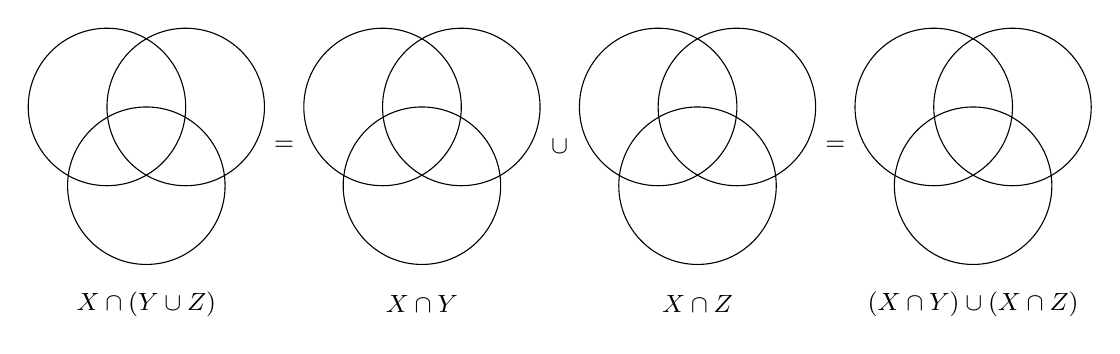
\begin{tikzpicture}[x=5mm, y=5mm,font=\small]

\draw (0,0) circle (2);
\draw (2,0) circle (2);
\draw (1,-2) circle (2);

\begin{scope}[xshift=35mm]
\draw (0,0) circle (2);
\draw (2,0) circle (2);
\draw (1,-2) circle (2);
\end{scope}

\begin{scope}[xshift=70mm]
\draw (0,0) circle (2);
\draw (2,0) circle (2);
\draw (1,-2) circle (2);
\end{scope}

\begin{scope}[xshift=105mm]
\draw (0,0) circle (2);
\draw (2,0) circle (2);
\draw (1,-2) circle (2);
\end{scope}

\foreach \x/\xtext in {4.5/=,11.5/\cup,18.5/=}
\node  at (\x,-1) {$\xtext$};

\foreach \xi/\xitext in {1/$X\cap(Y\cup Z)$,8/$X\cap Y$,15/$X\cap Z$,22/$(X\cap Y)\cup(X\cap Z)$}
\node  at (\xi,-5) {\xitext};
\end{tikzpicture}

\end{center}
\end{esercizio}

\begin{esercizio}
\label{ese:\thechapter.126}
Se~$E-F=E$ cosa puoi dire di~$E$ e~$F$?
\begin{center}
 \boxA\quad~$E\cup F=E$\quad\boxB\quad~$E=F$\quad\boxC\quad~$E\subseteq F$\quad\boxD\quad~$F\subset E$\quad\boxE\quad~$E\cap F=\emptyset $
\end{center}
\end{esercizio}

\begin{esercizio}
\label{ese:\thechapter.127}
Dimostra la proprietà distributiva dell'unione rispetto all'intersezione annerendo gli spazi opportuni
e inserendo le formule opportune.
\begin{center}
 % (c) 2012 Dimitrios Vrettos - d.vrettos@gmail.com
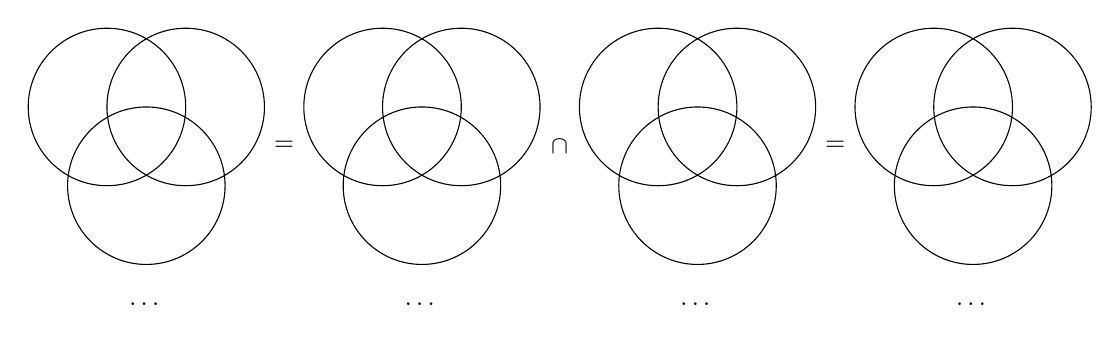
\begin{tikzpicture}[x=5mm, y=5mm,font=\small]

\draw (0,0) circle (2);
\draw (2,0) circle (2);
\draw (1,-2) circle (2);

\begin{scope}[xshift=35mm]
\draw (0,0) circle (2);
\draw (2,0) circle (2);
\draw (1,-2) circle (2);
\end{scope}

\begin{scope}[xshift=70mm]
\draw (0,0) circle (2);
\draw (2,0) circle (2);
\draw (1,-2) circle (2);
\end{scope}

\begin{scope}[xshift=105mm]
\draw (0,0) circle (2);
\draw (2,0) circle (2);
\draw (1,-2) circle (2);
\end{scope}

\foreach \x/\xtext in {4.5/=,11.5/\cap,18.5/=}
\node  at (\x,-1) {$\xtext$};

\foreach \xi in {1,8,15,22}
\node  at (\xi,-5) {\ldots};
\end{tikzpicture}

\end{center}
\end{esercizio}

\begin{esercizio}
\label{ese:\thechapter.128}
Quali dei seguenti sono sottoinsiemi dei numeri pari? L'insieme dei

\begin{center}
 \boxA\quad multipli di~4\quad\boxB\quad multipli di~3\quad\boxC\quad multipli di~6\quad\boxD\quad numeri primi
\end{center}
\end{esercizio}

\begin{esercizio}
\label{ese:\thechapter.129}
Dati gli insiemi~$A=\{x\mid x\in\insN$, $x<10\}$, $B=\{x\mid x\in\insN$, $5<x\le 16\}$ e
$C=\{x\mid x\in\insN$, $x\ge~7\}$ determina:
\begin{multicols}{4}
\begin{enumeratea}
\item $A\cup B\cup C$;
\item $A\cap B\cap C$;
\item $(A\cup B)\cap C$;
\item $(B\cap C)\cup A$.
\end{enumeratea}
\end{multicols}
\end{esercizio}

\begin{esercizio}
\label{ese:\thechapter.130}
Dati gli insiemi~$A=\{x\mid x\in\insQ$, $3<x\le 10\}$, $B=\{x\mid x\in\insQ$, $x>3\}$ e
$C=\{x\mid x\in\insQ$, $x\le~5\}$ determina:
\begin{multicols}{3}
\begin{enumeratea}
\item $A\cup B$;
\item $A\cap C$;
\item $B-A$;
\item $A\cup B\cup C$;
\item $A\cap B\cap C$;
\item $(A\cup B)\cup C$.
\end{enumeratea}
\end{multicols}
\end{esercizio}

\begin{esercizio}
\label{ese:\thechapter.131}
Dati gli insiemi~$A=\{x\mid x\in\insQ$, $x<10\}$, $B=\{x\mid x\in\insQ$, $7\le x<20\}$ e
$C=\{x\mid x\in\insQ$, $x\ge~20\}$ calcola:
\begin{multicols}{3}
\begin{enumeratea}
\item $B\cup C$;
\item $B\cap C$;
\item $A\cap C$;
\item $C-B$;
\item $\overline{A}$;
\item $\overline{A\cap C}$;
\item $B-C$;
\item $A\cup B$;
\item $A\cap \overline{C}$.
\end{enumeratea}
\end{multicols}
\end{esercizio}

\begin{esercizio}
\label{ese:\thechapter.132}
Dato~$A = \{x\mid x$ è un numero naturale, $x$ è pari e $x>12\}$ determina l'insieme complementare di~$A$.
\end{esercizio}

\begin{esercizio}
\label{ese:\thechapter.133}
Quanti sono i sottoinsiemi dell'insieme che contiene come elemento
l'insieme vuoto?
\end{esercizio}

\begin{esercizio}
\label{ese:\thechapter.134}
Dati $A=\{x\mid x$ è divisore di~12$\}$, $B=\{x\mid x$ è divisore di~6$\}$ e
$C=\{x\mid x$ è divisore di~15$\}$, determina:
\begin{multicols}{4}
 \begin{enumeratea}
 \item $A\cup B$;
 \item $A\cup C$;
 \item $A\cup B\cup C$;
 \item $A\cap B$;
 \item $B\cap C$;
 \item $A\cap C$;
 \item $A\cap B\cap C$;
 \item $A\cap(B\cup C)$.
 \end{enumeratea}
\end{multicols}
\end{esercizio}

\begin{esercizio}
\label{ese:\thechapter.135}
Dato l'insieme~$U=\{x\mid x=2n+1$, $n\in\insN$, $0\le n\le~5\}$:

\begin{enumeratea}
\item rappresenta~$U$ in forma tabulare;
\item costruisci due sottoinsiemi propri~$A$ e~$B$ di~$U$ tali che~$A\cap B=\emptyset $;
\item determina~$A\cup B$ e~$A-B$, dai il risultato con rappresentazione tabulare e mediante diagrammi di
Eulero-Venn.
\end{enumeratea}
\end{esercizio}

\begin{esercizio}
\label{ese:\thechapter.136}
In base agli insiemi rappresentati con il diagramma di Eulero-Venn nella figura determina gli insiemi richiesti:
\begin{multicols}{2}
\begin{enumeratea}
\item $A\cup B$;
\item $\overline{A\cup B\cup C}$;
\item $A\cap B$;
\item $B\cap C$;
\item $A\cap B\cap C$;
\item $A\cap (B\cup C)$;
\item $A\cup (B\cap C)$;
\item $B\cap \overline{C}$;
\item $(A\cup B)-C$;
\item $B\cap \overline{C}$
\item $C-(A\cap B)$;
\item $\overline{(A\cup B)}-C$.
\end{enumeratea}
\begin{center}
 % (c) 2012 Dimitrios Vrettos - d.vrettos@gmail.com
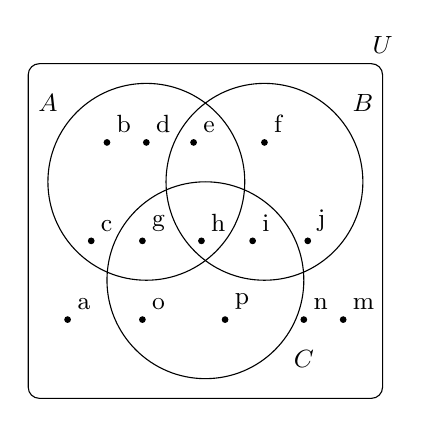
\begin{tikzpicture}[x=5mm, y=5mm,font=\small]

\draw[rounded corners] (-4,-5.5) rectangle (5,3) node[above] {$U$};
\draw (-1,0) circle (2.5) (-3.5,2)node {$A$};
\draw (2,0) circle (2.5) (4.5,2)node {$B$};
\draw (0.5,-2.5) circle (2.5) (3,-4.5)node {$C$};

\foreach \x/\xtext in {-2/b,-1/d,0.2/e,2/f}
\draw[fill] (\x,1)circle(1pt) node[above right]{\xtext};

\foreach \x/\xtext in {-2.4/c,-1.1/g,0.4/h,1.7/i, 3.1/j}
\draw[fill] (\x,-1.5)circle(1pt) node[above right]{\xtext};

\foreach \x/\xtext in {-3/a,-1.1/o,1/p,3/n, 4/m}
\draw[fill] (\x,-3.5)circle(1pt) node[above right]{\xtext};
\end{tikzpicture}

\end{center}
\end{multicols}
\end{esercizio}

\begin{esercizio}
\label{ese:\thechapter.137}
Determina l'insieme~$\wp(A)$, insieme delle parti di~$A$, dove $A$ è l'insieme delle lettere della parola ``NONNA''.
\end{esercizio}

\begin{esercizio}
\label{ese:\thechapter.138}
Nel seguente diagramma di Eulero-Venn gli insiemi~$r$, $s$, $t$
sono rette, gli elementi~$A$, $B$, $C$, $D$ sono punti. Dai una
rappresentazione geometrica, individuando le rette che corrispondono
alla seguente situazione.

\begin{center}
 % (c) 2012 Dimitrios Vrettos - d.vrettos@gmail.com
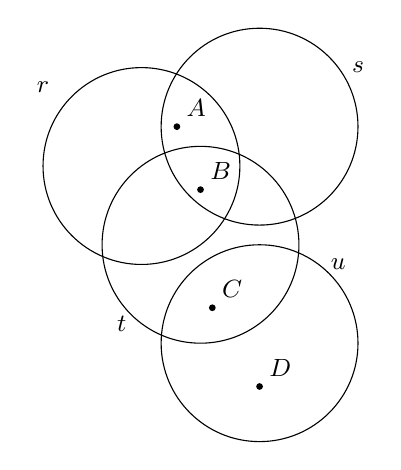
\begin{tikzpicture}[x=5mm, y=5mm,font=\small]
\draw (-1,0) circle (2.5) (-3.5,2)node {$r$};
\draw (2,1) circle (2.5) (4.5,2.5)node {$s$};
\draw (0.5,-2) circle (2.5) (-1.5,-4)node {$t$};
\draw (2,-4.5) circle (2.5) (4,-2.5)node {$u$};

\draw[fill] (-.1,1) circle (1pt) node[above right]  {$A$};
\draw[fill] (.5,-.6) circle (1pt) node[above right]  {$B$};
\draw[fill] (.8,-3.6) circle (1pt) node[above right]  {$C$};
\draw[fill] (2,-5.6) circle (1pt) node[above right]  {$D$};
\end{tikzpicture}

\end{center}
\end{esercizio}

\subsection{Risposte}
\begin{multicols}{2}
\paragraph{\thechapter.46.} a)~16,\quad b)~20,\quad c)~10,\quad d)~14.

\paragraph{\thechapter.78.} 46.

\paragraph{\thechapter.80.} 3; A.

\paragraph{\thechapter.81.} 22.

\paragraph{\thechapter.82.} a)~$\np{1048}$,\quad b)~$\np{1279}$,\quad c)~$\np{1350}$.

\paragraph{\thechapter.83.} 36; 84.
\end{multicols}

\cleardoublepage
